\documentclass{article}

\usepackage[margin=2.5cm]{geometry}

\usepackage[utf8]{inputenc}
\usepackage[T1]{fontenc}
\usepackage[german]{babel}

\usepackage{hyperref}
\hypersetup{
pdftitle={Pflichtenheft},
bookmarks = true
}
\usepackage[toc]{glossaries}

\usepackage{graphicx}

\usepackage[shortlabels]{enumitem}
\usepackage{parskip}

\usepackage{float}
\floatplacement{figure}{H}
\usepackage{placeins}

\usepackage{amsmath}
\usepackage{amssymb}

%\usepackage{svg}
%\usepackage{algpseudocode}
%\usepackage{algorithm}
\usepackage{caption}
\usepackage{subcaption}
%\usepackage{fancyvrb}
%\usepackage{tgcursor}
%\fvset{frame=single,framesep=1mm,fontfamily=courier,fontsize=\scriptsize,numbers=left,framerule=.3mm,numbersep=1mm,commandchars=\\\{\}}




\usepackage{fix-cm}
\newcommand{\titlesize}{\fontsize{30pt}{20pt}\selectfont}
\newcommand{\themesize}{\fontsize{20pt}{20pt}\selectfont}
\newcommand{\authorsize}{\fontsize{15pt}{20pt}\selectfont}

\newcommand{\mypackage}[1]{\subsection*{Package #1} \label{#1} \addcontentsline{toc}{subsection}{\nameref{#1}}}
\newcommand{\myclass}[1]{\subsubsection*{Class #1} \label{#1} \addcontentsline{toc}{subsubsection}{\nameref{#1}}}
\newcommand{\myinterface}[1]{\subsubsection*{Interface #1} \label{#1} \addcontentsline{toc}{subsubsection}{\nameref{#1}}}

%\makeglossaries



%\titlehead{\centering 
\includegraphics{images/title}}
%\title{RaGE Pflichtenheft}
%\author{Jonas Kasper, Bernard Hohmann, Thomas Fischer, Christian Jung, Jonas Linßen}

\begin{document}
	%\maketitle
	
	%\newpage
	
	\begin{titlepage}
		%\centering 
\includegraphics[width=0.7\textwidth]{images/title}
		
		\titlesize \hspace*{.5cm} Random Graph Coloring Evaluation
		~\newline~\newline
		
		\themesize \hspace*{3cm} Entwurfsdokument
		\newline~\newline
		
		\authorsize Jonas Kasper, Bernard Hohmann, Thomas Fischer, Christian Jung, Jonas Linßen
	\end{titlepage}
	
	\tableofcontents
	\newpage
	
	\section{Anmerkungen zum Pflichtenheft}
	\subsection{Klarstellungen}
	\subsection{Änderungen}	
	\subsubsection{GUI}
			%\begin{enumerate}
			\paragraph{Graphen-Vorschau}
				%Worum geht es?
				In der Graph-Preview Ansicht in der GUI werden die einzelnen Graphen, seien sie generiert oder importiert, unter einem neuen Tab angezeigt.
				
				%Wie war es bisher?
				Diese Anzeige war bisher so gestaltet, dass die Graphen in einer Grid-View gesetzt werden.
				Dies würde in einer tabellenartigen Darstellung resultieren, bei der Beispielsweise 2 Spalten und 3 Reihen für die Graphen gleichzeitig dargestellt werden.
				
				%Was war Grund der Änderung:
				Diese Ansicht hatte den Nachteil, dass der User immer gezeichnete Graphen vor sich sieht.
				Dies führt zu deutlich geringerer Übersichtlichkeit.
				Außerdem bestand kein großes Interesse des Kunden daran, dass man die zuvor generierten Graphen sofort betrachten kann.
					Das graphische Darstellen der Graphen wurde eher an anderer Stelle gewünscht.
				Darüber hinaus ist diese Art der Ansicht nicht besonders gut skalierbar, wenn der User die Fenstergröße anpassen möchte, besteht die Gefahr, dass die Graphen-Bilder zu klein werden, um anschaulich zu sein.
				
				%Was ist die Änderung?
				Aus diesem Grund haben wir die Ansicht zu einer Tab-View geändert.
				Dies bedeutet, dass man nun eine Liste an ausklappbaren Tabs mit den jeweiligen Graphen-Namen vor sich sieht.
				Demzufolge kann man bei Interesse die Graphen-Tabs ausklappen.
					Beim Ausklappen wird dann genau dieser zu betrachtende Graph gezeichnet.
					Daraus folgt, dass man nicht mehr mit Graphen-Zeichnungen überschüttet wird.
				
				%Folgen für das weitere Programm
				Durch diese Änderung entsteht ein weiterer Vorteil.
				Die Performance des Programms wird verbessert, da das Programm nicht sofort alle Graphen zeichnen muss, sondern diesen Task erst bei Bedarf starten muss.
			
		
		\paragraph{Graphen-Generierung}
			%Worum geht es?
			Möchte man die Heuristiken anwenden, benötigt man selbstverständlich hierfür erst einmal Graphen.
			Unser Programm stellt zu diesem Zweck mehrere Beschaffungsmöglichkeiten zur Verfügung:
				Automatische zufällige Generierung mit zuvor getätigten Einstellungen.
				Import bereits generierter Graphen.
				Im Graph-Editor von Grund auf neue Graphen von Hand erstellen.
			
			%Wie war es bisher?
			Unter dem Tab "Graphen Generieren" der GUI war es bisher so gehalten, dass man als erstes die möglichen Einstellungsmöglichkeiten zur Generierung hat und sich darunter dann die verschiedenen Knöpfe befinden, welche die Generierung, den Import, oder das Zeichnen von Hand starten.
			
			%Was war Grund der Änderung:
			Diese Anordnung macht nur wenig Sinn, da man im Falle eines Imports oder auch des Editors keine Einstellungsmöglichkeiten benötigt.
			
			%Was ist die Änderung?
			Aus diesem Grund befinden sich nun die Buttons, welche die einzelnen möglichen Aktionen (Starten der Generierung, des Zeichnens oder Imports) ausführen, an oberster Stelle.
			Außerdem werden die Einstellungsmöglichkeiten zur zufälligen Generierung so lange vor dem User verborgen, bis er/sie aktiv auswählt diese Funktionalität wirklich zu benutzen.
		
	
		\paragraph{Graphen-Editor}
			%Worum geht es?
			Beim Graph-Editor kann man standardmäßig sowohl einen „Simple-Undirected-Graph“, als auch „Simple-Hyper-Graph“ editieren oder auch erstellen.
			Dabei gibt es unterschiedliche Funktionen, die dem User geboten werden um dies zu tun.
			
			%Wie war es bisher?
			Bisher wurden diese nicht auf spezielle Graphentypen eingeschränkt.
			
			%Was war Grund der Änderung:
			Allerdings entsteht bei einigen der angebotenen Funktionen die Gefahr, dass der User den Graphentyp durch die gemachten Änderungen verändert, oder gar den gesamten Graphen ungültig für die weitere Bearbeitung macht.
			
			%Was ist die Änderung?
			Die daraus von uns getroffene Anpassung war es die Funktionen auf den Graphen-Typ einzuschränken und den Graph-Editor den Typ des editierten Graphen überprüfen zu lassen.
		
		%\end{enumerate}	
		\section{Übersicht}
	\subsection{Architektur}
	Das System basiert auf dem Model-View-Controller(MVC)-Muster mit einer drei-Schichten-Architektur und einer durch JavaFX realisierten graphischen Benutzerschnittstelle.\\	
	 Beim MVC-Muster wird das System in die drei Komponenten Modell, Präsentation und Steuerung aufgeteilt.\\
	Das Modell (Model) enthält und verarbeitet die Daten, welche dann von der Präsentation (View) dargestellt werden. Die Steuerung (Controller) steuert den Ablauf und das Verhalten der Anwendung. Dafür werden Benutzereingaben auf Modeländerungen und Ausführung von Berechnungen abgebildet. Weiterhin informiert das Model direkt oder über den Controller die View über Änderungen am Model (z.B. Ergebnisse von Berechnungen) und sorgt damit für eine Anpassung bzw. Aktualisierung der View.\\
	In der hier verwendeten Architektur erfolgt die Kommunikation zwischen View und Model immer über den Controller. Dabei gibt es \texttt{FXController}-Komponenten, welche die Steuerung der View übernehmen, und \texttt{Controller}-Komponenten, welche als Schnittstelle zwischen den \texttt{FXControllern} und dem Model dienen.\\
	Dadurch kann das System in drei logische Schichten unterteilt werden, eine Daten-, eine Logik- und eine Benutzerschicht \ref{img:struktur}.
	%Diese Architektur ist durch Erweiterung bzw. einen Austausch der \textbf{Controller}-Komponenten auch in eine physisch getrennte drei-Schichten-Architektur überführbar.\\
		
	
	
	
	\begin{figure}
	\centering
	%\fbox{
	%\begin{subfigure}[t]{0.4\textwidth}
%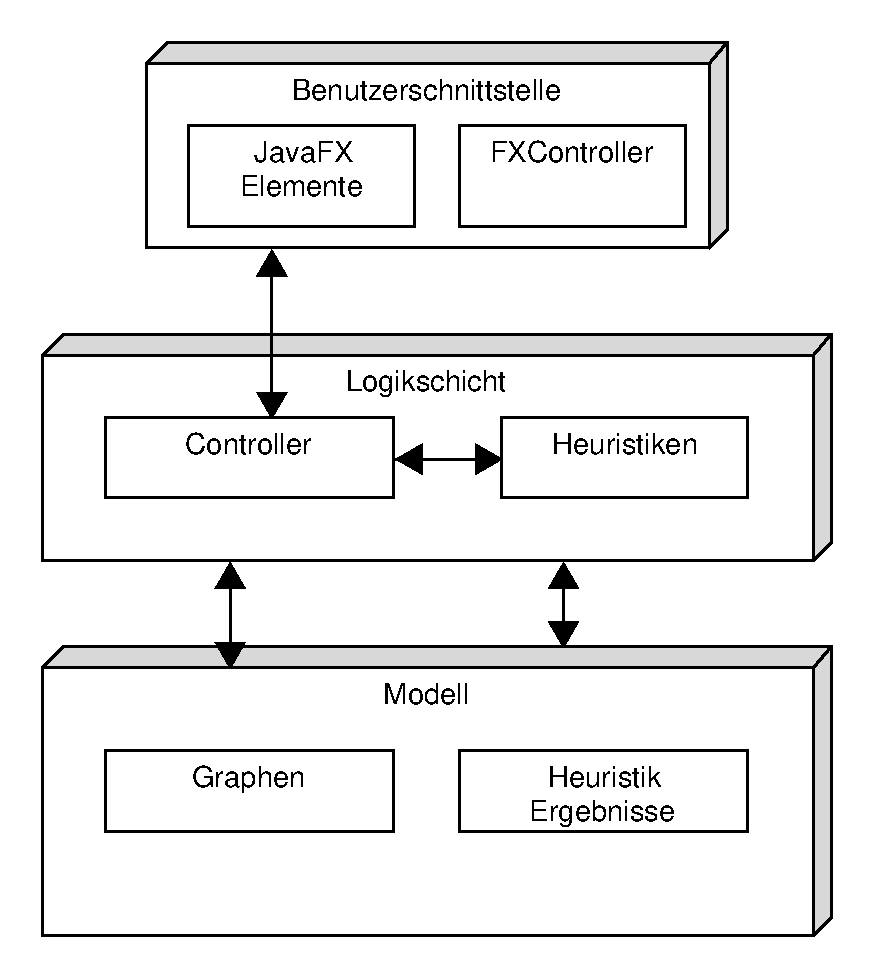
\includegraphics[height=2.8in]{struktur2.pdf}
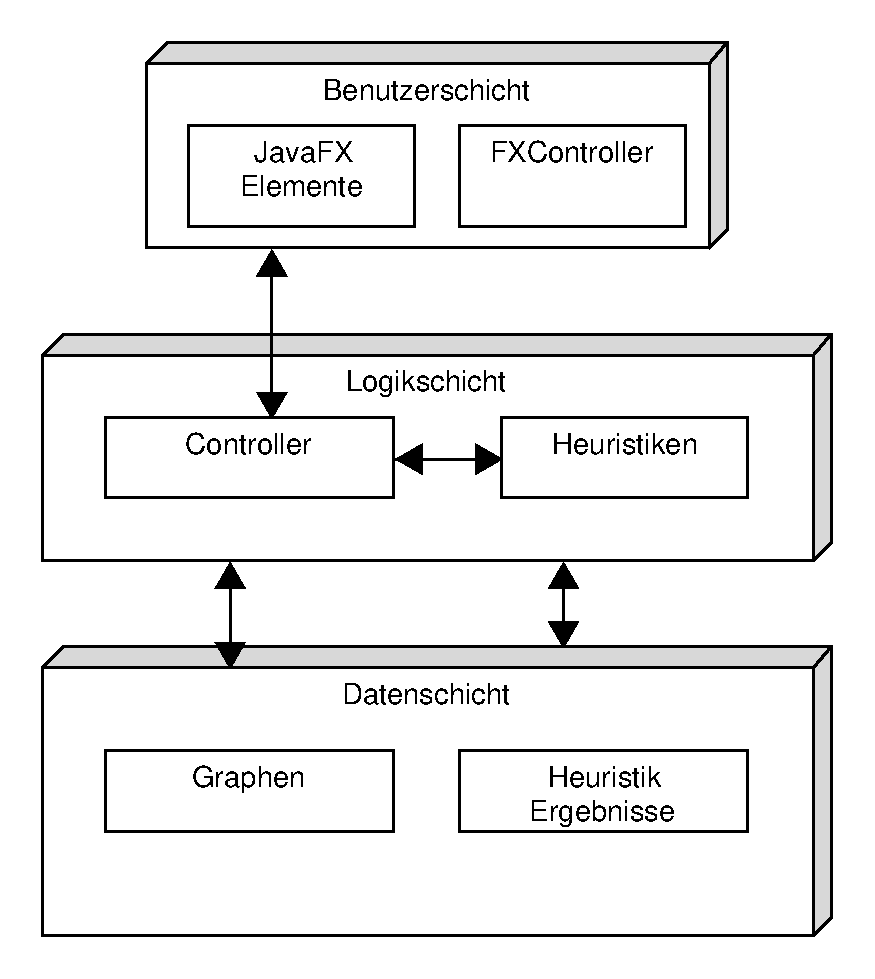
\includegraphics[height=2.8in]{abbildungen/struktur3.pdf}

%\subcaption{Darstellung als Schichtenarchitektur.}
%\end{subfigure}
	%\begin{subfigure}[t]{0.4\textwidth}
%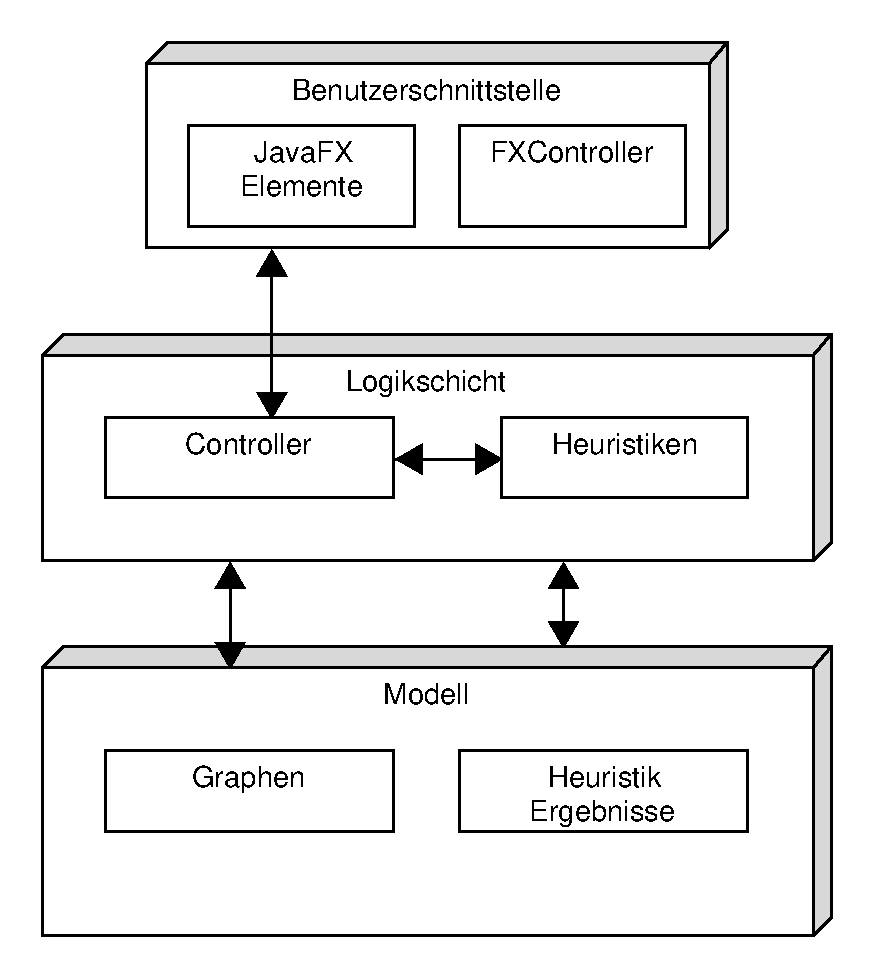
\includegraphics[height=2.8in]{struktur2.pdf}
%\subcaption{Model-View-Controller.}
%\end{subfigure}
%   }
	\caption{Die Architektur als drei-Schichtenmodell }
	\label{img:struktur}
\end{figure}

\subsection{Sequenzdiagramme}
Durch Benutzereingaben initiierte Aktionen werden durch das JavaFX-Framework an die entsprechenden \texttt{FXController} weitergeleitet. (TODO wie werden Controller und Aktionen verbunden?). Dieses wird in den folgenden Diagrammen deshalb nicht dargestellt, sondern nur die anschließenden Interaktionen.
\subsubsection{Heuristiken ausführen}
	Eine Benutzereingabe zum Ausführen der Ausgewählten Heuristiken wird durch den \texttt{FXTabController} verarbeitet und and den \texttt{TabController} weitergeleitet. Zu jeder ausgewählten Heuristik wird die Methode \mbox{\texttt{addToHeuristic}} aufgerufen. Diese erzeugt zuerst ein Objekt der entsprechenden Heuristik. Diese wird zum \texttt{DataPool}, welcher Graphen mit darauf auszuführenden Heuristiken enthält, hinzugefügt. Dabei wird beim Hinzufügen die Heuristik über die \texttt{applyTo}-Methode auf alle Graphen im \texttt{DataPool} angewandt.\\
	Ist die Anwendung aller Heuristiken abgeschlossen, wird eine Liste von Ergebnissen der Berechnungen vom Typ \texttt{HeuristicResult} vom \texttt{DataPool} zurückgegeben und über den \texttt{TabController} an den \texttt{FXTabController} weitergeleitet.
	
	\begin{figure}
	\centering
	%\fbox{	
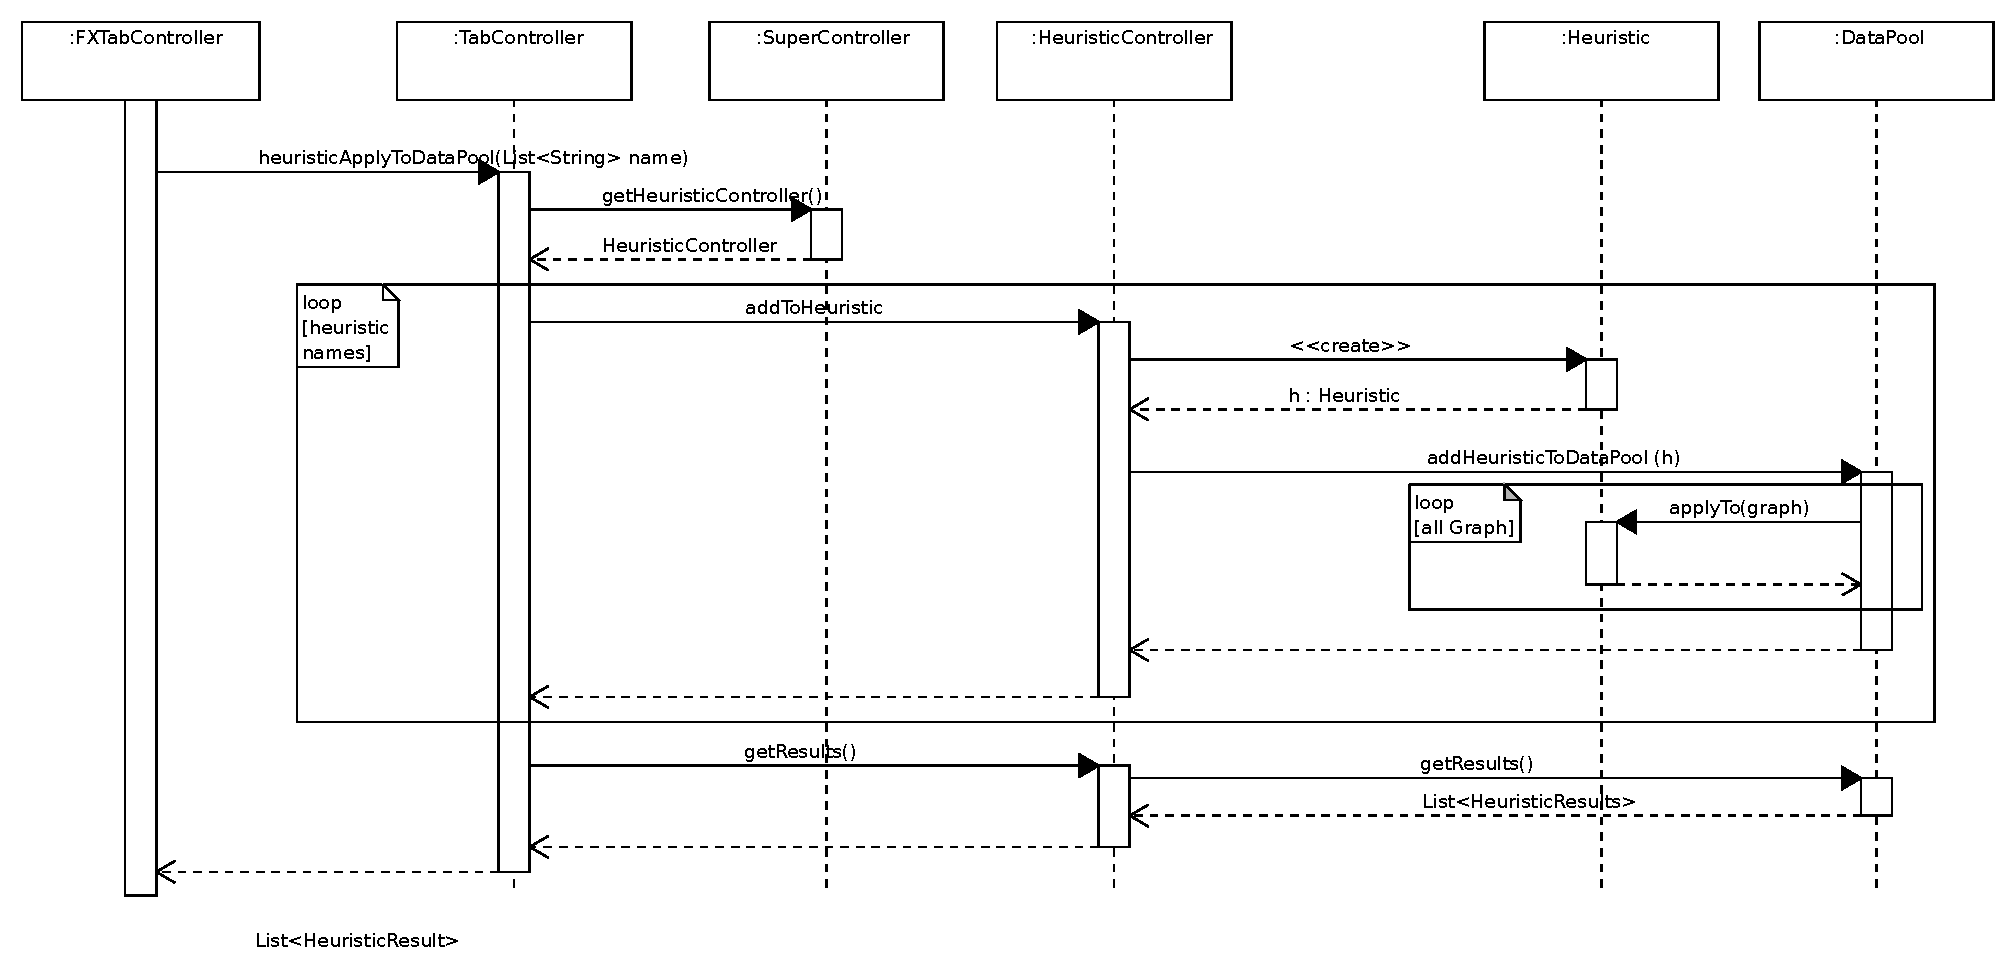
\includegraphics[width=\textwidth]{abbildungen/heuristik-seq.pdf}
\caption{Sequenzdiagramm zum Ausführen von Heuristiken }
	\label{img:heuristic-seq}
	\end{figure}
\subsubsection{Graphen generieren}
Eine Benutzereingabe zum Generieren von Graphen wird vom \texttt{FXGraphGeneratorController} verarbeitet. Dieser delegiert durch den Aufruf der Methode \texttt{generate} an den \texttt{GraphGeneratorController}. Hier wird für alle $n$ zu generierenden Graphen durch die Klasse \texttt{GraphBuilder} jeweils ein Objekt vom Typ \texttt{Graph} erzeugt und zu einem \texttt{DataPool} hinzugefügt. Jeder dieser Graphen wird anschließend durch die Klasse \texttt{GraphAdapter} in eine für die View benötigte Graphenstruktur umgewandelt.\\
Nach Generierung der Graphen wird ein neuer \texttt{TabController} erzeugt. Diesem wird der \texttt{DataPool} der neu generierten Graphen übergeben. Zum Schluss wird noch ein neuer \texttt{FXTabController} erzeugt, welcher für die Anzeige des Tabs für die generierten Graphen zuständig ist.

\begin{figure}
	\centering
	%\fbox{	
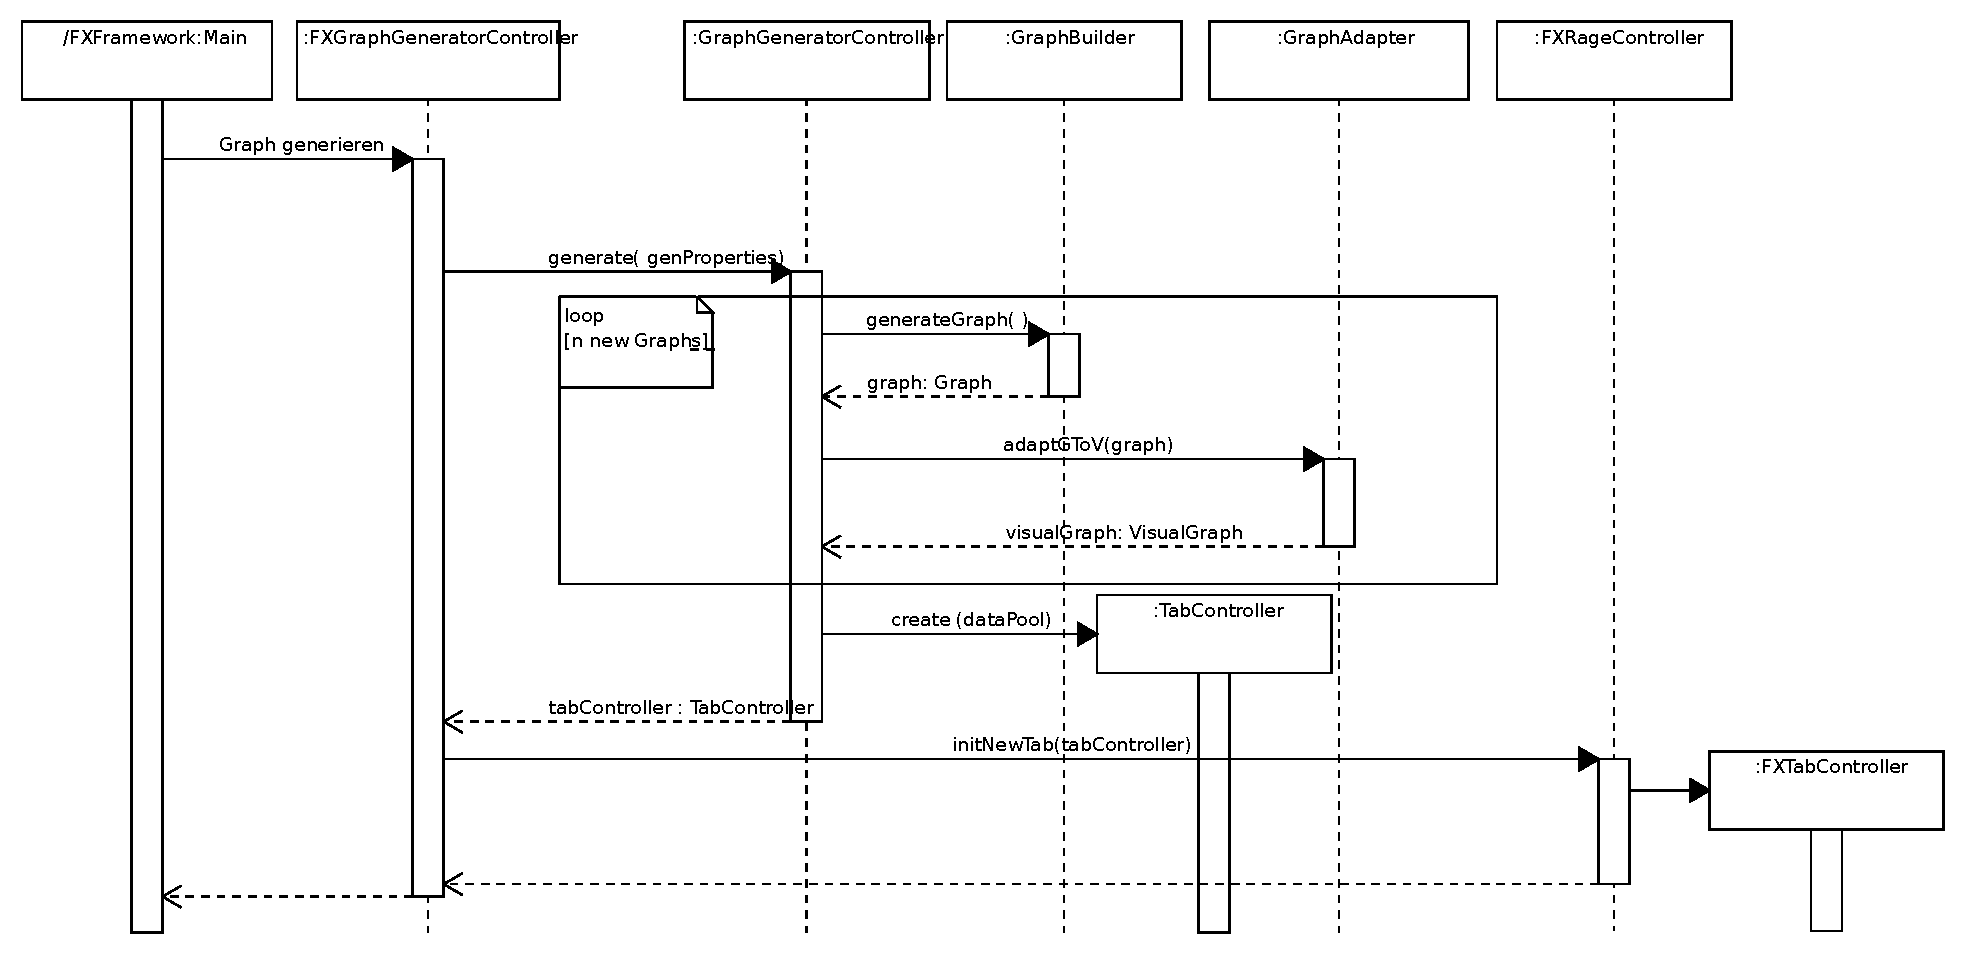
\includegraphics[width=\textwidth]{abbildungen/graphgen-seq.pdf}
\caption{Sequenzdiagramm zum Generieren von Graphen }
	\label{img:graphgen-seq}
	\end{figure}
	
	\subsubsection{Graphen modifizieren}
	Das Modifizieren von Graphen erfolgt über die Detailansicht des Graphen. Dafür wird zuerst ein \newline \texttt{FXDetailViewController} erzeugt. Bekommt dieser anschließend eine Benutzereingabe zum Modifizieren, dann wird ein \texttt{FXGraphEditorController}-Objekt erzeugt. Den dafür benötigten \texttt{GraphEditorConroller} erhält er über den Aufruf der Methode \texttt{getGEC} des \texttt{SuperControllers}.\\
	Anschließende Editierbefehle werden direkt an den \texttt{FXGraphEditorController} weitergeleitet und von diesem verarbeitet. Bei Abschluss des Editieren durch den Benutzer wird der modifizierte Graph als neuer Graph durch den \texttt{GraphEditorController} zum \texttt{DataPool} hinzugefügt.
\begin{figure}
	\centering
	%\fbox{	
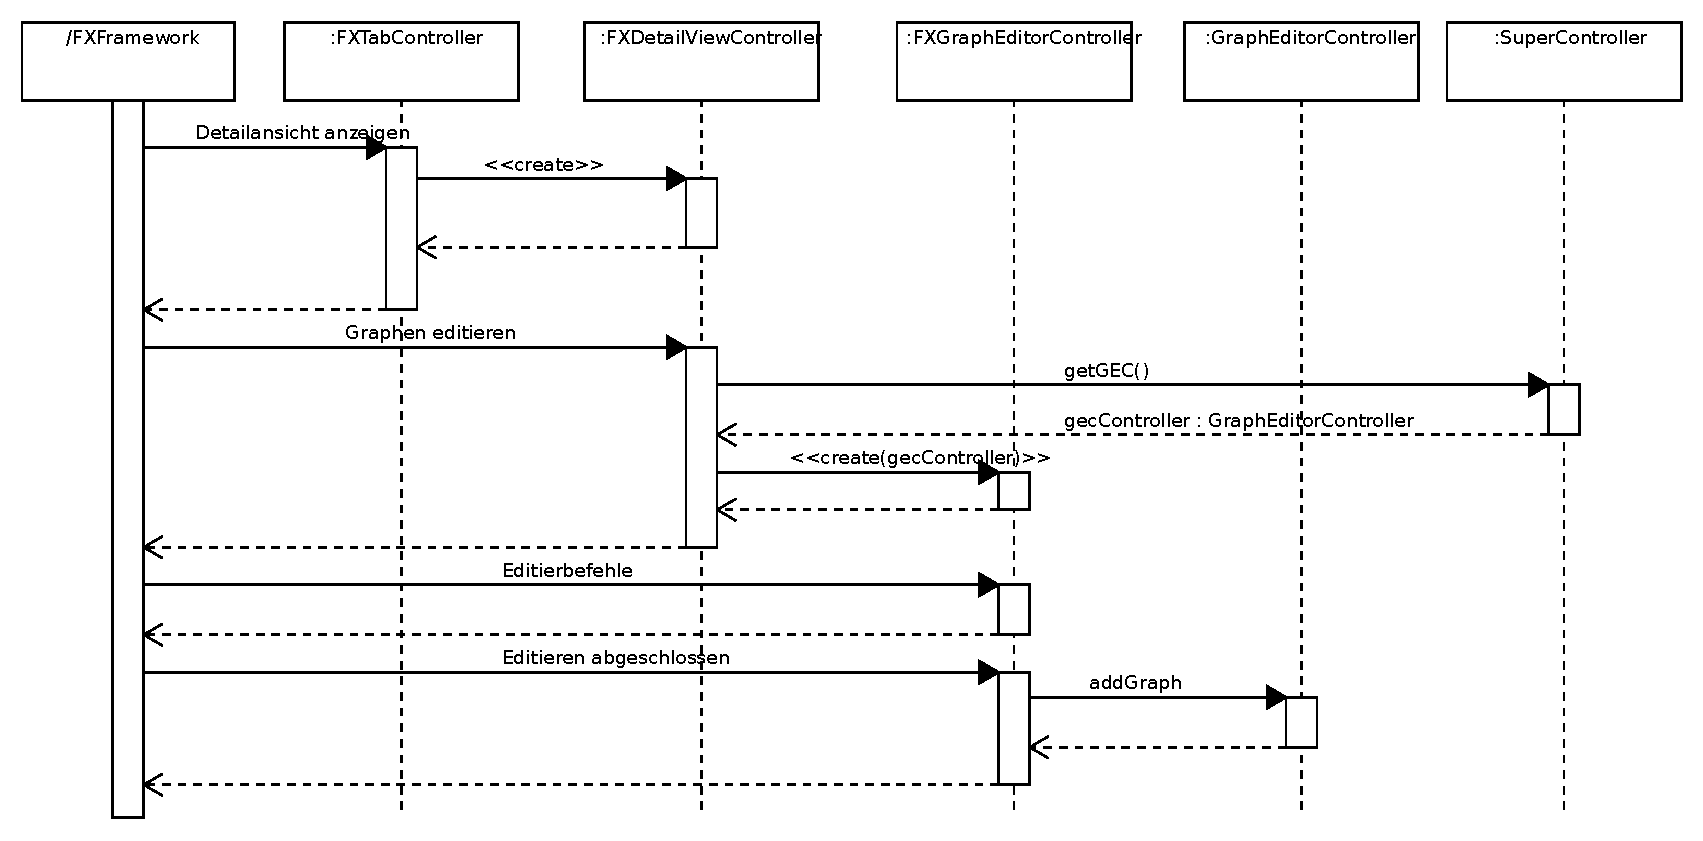
\includegraphics[width=\textwidth]{abbildungen/graphmod-seq.pdf}
\caption{Sequenzdiagramm zum Modifizieren von Graphen }
	\label{img:grapmod-seq}
	\end{figure}
	
	~\newpage
		\section{Model}
	
	\mypackage{graph}
	This package contains the interfaces for the interaction with graphs. In the subpackages concrete graph-types are implemented.
	
		\begin{figure}
	\centering
	%\fbox{	
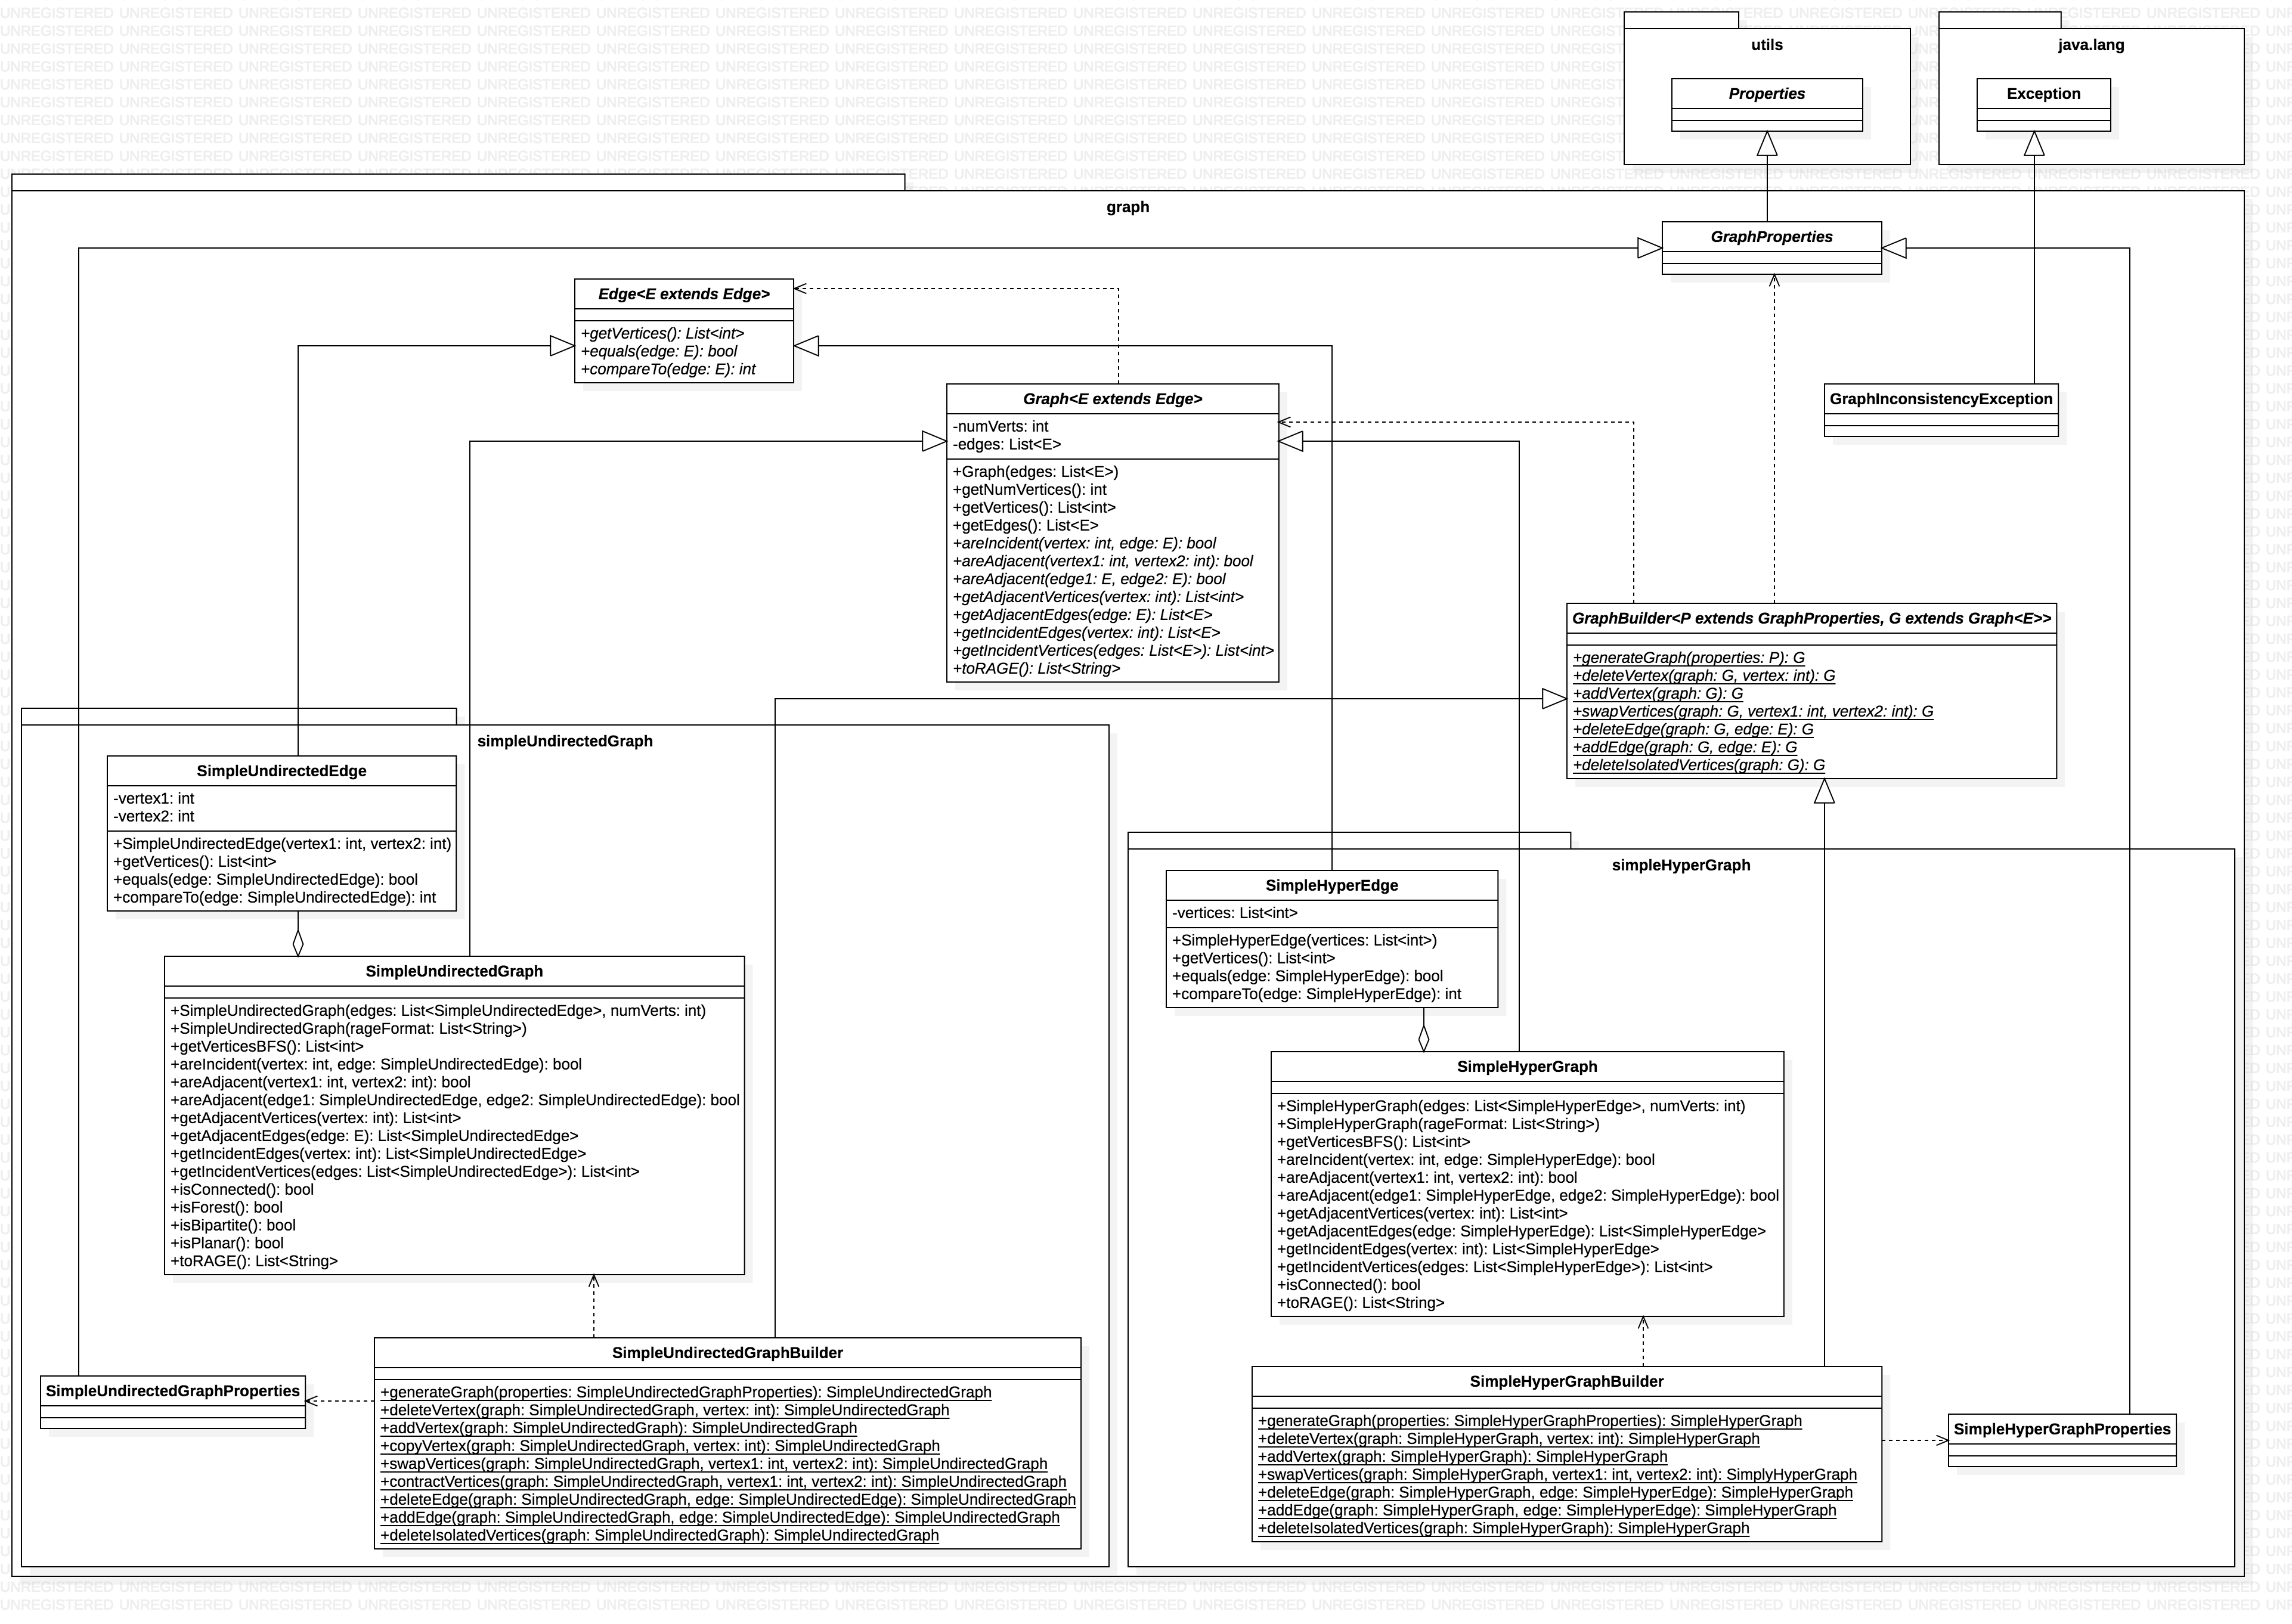
\includegraphics[width=\textwidth]{abbildungen/graph.png}

	\caption{Das Paket graph }
	\label{img:graph}
\end{figure}		
	
	
	\myclass{Graph}
	\textbf{Description}
	
	This class describes the abstract structure of a graph. Each graph has (independent of its concrete type) a finite amount of vertices and edges, which define a relation of vertices. The type \textbf{E} of this edges defines the concrete graph type. The class has methods for retrieving the relations given by the edges. Vertices are identified with their unique index and thus are not saved explicitly.
	
	\textbf{Documentation}
	\begin{enumerate}[+]
		\item{
			\textbf{Graph(edges: List<E>, numVertices: int)} \newline
			the constructor of this class \newline
			\textbf{@param edges} the edges belonging to this graph
			\textbf{@numVertices} the number of vertices this graph has
		}
		\item{
			\textbf{getNumVertices(): int} \newline
			\textbf{@return} returns the number of vertices which the graph contains
		}
		\item{
			\textbf{getVertices(): int} \newline
			convenience method for retrieving the list of vertex indices \newline
			\textbf{@return} returns the list [0 ... numVertices$-1$]
		}
		\item{
			\textbf{getEdges(): List<E>} \newline
			\textbf{@return} returns the edges giving the graph its structure
		}
		\item{
			\textbf{areIncident(vertex: int, edge: E): bool} \newline
			\textbf{@param vertex} the index of a vertex of the graph ie. in [0 ... numVertices$-1$]\newline
			\textbf{@param edge} an edge of the graph \newline 
			\textbf{@return} returns \textbf{true} iff the vertex is incident to the given edge \newline
			\textbf{@throws GraphInconstistencyException} if \textbf{vertex} is an invalid vertex index or \textbf{edge} is not an edge of the graph
		}
		\item{
			\textbf{areAdjacent(vertex1: int, vertex2: int): bool} \newline
			\textbf{@param vertex1} the index of a vertex of the graph ie. in [0 ... numVertices$-1$] \newline
			\textbf{@param vertex2} see \textbf{vertex1} \newline
			\textbf{@return} returns \textbf{true} iff there is an edge which is incident to both vertices \newline
			\textbf{@throws GraphInconsistencyException} if \textbf{vertex1} or \textbf{vertex2} is not a valid vertex index
		}
		\item{
			\textbf{areAdjacent(edge1: E, edge2: E): bool} \newline
			\textbf{@param edge1} an edge of the graph \newline
			\textbf{@param edge2} another edge of the graph \newline
			\textbf{@return} returns \textbf{true} iff there is a vertex which is incident to both edges \newline
			\textbf{@throws GraphInconsistencyException} if \textbf{edge1} or \textbf{edge2} is not an edge of the graph
		}
		\item{
			\textbf{getAdjacentVertices(vertex: int): List<int>} \newline
			\textbf{@param vertex} the index of a vertex of the graph ie. in [0 ... numVertices$-1$] \newline
			\textbf{@return} returns the list of all vertices which are adjacent to \textbf{vertex} \newline
			\textbf{@throws GraphInconsistencyException} if \textbf{vertex} is not a valid vertex index
		}
		\item{
			\textbf{getAdjacentEdges(edge: E): bool} \newline
			\textbf{@param edge} an edge of the graph \newline
			\textbf{@return} returns the list of all edges which are adjacent to \textbf{edge} \newline
			\textbf{@throws GraphInconsistencyException} if \textbf{edge} is not an edge of the graph
		}
		\item{
			\textbf{getIncidentEdges(vertex: int): List<E>} \newline
			\textbf{@param vertex} the index of a vertex of the graph ie. in [0 ... numVertices$-1$] \newline
			\textbf{@return} returns the list of all edges incident to \textbf{vertex} \newline
			\textbf{@throws GraphInconsistencyException} if \textbf{vertex} is an invalid vertex index
		}
		\item{
			\textbf{getIncidentVertices(edges: List<E>): List<int>} \newline
			\textbf{@param edges} a list of edges of the graph \newline
			\textbf{@return} returns the list of all vertices which are incident to any of the edges in the list \newline
			\textbf{@throws GraphInconsistencyException} if there is an edge in \textbf{edges}, which is not an edge of the graph
			
		}
		\item{
			\textbf{\textit{toRAGE(): List<String>}} \newline
			\textbf{@return} returns the line-by-line representation of the graph as specified in the RAGE-data format
		}
	\end{enumerate}
	
	~\newline
	~\newline
	~\newline
	
	\myclass{Edge}
	\textbf{Description}
	
	An edge always defines an adjacency-relation of the vertices incident to it. Moreover this class provides methods to compare edges.
	
	\textbf{Documentation}
	\begin{enumerate}[+]
		\item{
			\textbf{\textit{getVertices(): List<int>}} \newline
			\textbf{@return} returns the list of all indices of vertices incident to this edge
		}
		\item{
			\textbf{\textit{equals(edge: E): bool}} \newline
			\textbf{@return} returns \textbf{true} iff \textbf{edge} equals the edge this method is invoked upon. Note that the notion of equality depends on the concrete implementation.
		}
		\item{
			\textbf{\textit{compareTo(edge: E): int}} \newline
			\textbf{@return} returns \textbf{-1}/\textbf{0}/\textbf{1} if \textbf{edge} is greater/equal/smaller than the edge this method is invoked upon. Note that the notions of order and equality depend on the concrete implementation.
		}
	\end{enumerate}
	
	\newpage
	
	\myclass{GraphProperties}
	
	\textbf{Description}
	
	This class is required for exchanging data between controller and model, especially to signal the settings required to generate graphs. It assures that the following graph-properties can be retrieved and set at all times:
	
	\begin{enumerate}[--]
		\item{''graphTypes'' -- a const list of strings, initialised with [''simpleUndirectedGraph'', ''simpleHyperGraph'']}
		\item{''type'' -- a string}
		\item{''numVertices'' -- a nonnegative integer}
	\end{enumerate}
	
	~\newline
	~\newline
	~\newline
	
	\myclass{GraphBuilder}
	
	\textbf{Description}
	This class is a factory class to generate graphs of type \textbf{G} by given GraphProperties \textbf{G} as well as to modify graphs of this type.
	
	\textbf{Documentation}
	\begin{enumerate}[+]
		\item{
			\textbf{\textit{generateGraph(properties: P): G}} \newline
			\textbf{@param properties} the properties which the generated graphs will have \newline
			\textbf{@return} returns a randomly generated graph satisfying the specified \textbf{properties}
		}
		\item{
			\textbf{\textit{deleteVertex(graph: G, vertex: int): G}} \newline
			\textbf{@param graph} the graph which is going to be modified \newline
			\textbf{@param vertex} the index of a vertex of \textbf{graph}, which will be deleted \newline
			\textbf{@return} returns a modified copy of \textbf{graph} in which the vertex with index \textbf{vertex} and all edges incident to it are deleted \newline
			\textbf{@throws GraphInconsistencyException} if \textbf{graph} has no vertex with index \textbf{vertex} 
		}
		\item{
			\textbf{\textit{addVertex(graph: G): G}} \newline
			\textbf{@param graph} the graph which is going to be modified \newline
			\textbf{@return} returns a modified copy of \textbf{graph} which has precisely one isolated vertex more
		}
		\item{
			\textbf{\textit{swapVertices(graph: G, vertex1: int, vertex2: int): G}} \newline
			\textbf{@param graph} the graph which is going to be modified \newline
			\textbf{@param vertex1} the index of a vertex of \textbf{graph} \newline
			\textbf{@param vertex2} the index of another vertex of \textbf{graph} \newline
			\textbf{@return} returns a modified copy of \textbf{graph} in which the vertices having index \textbf{vertex1} and \textbf{vertex2} swap indices. Note this results in a different but isomorphic graph to \textbf{graph}  \newline
			\textbf{@throws GraphInconsistencyException} if \textbf{graph} has no vertex with index \textbf{vertex1} or \textbf{vertex2} 
		}
		\item{
			\textbf{\textit{deleteEdge(graph: G, edge: E): G}} \newline
			\textbf{@param graph} the graph which is going to be modified \newline
			\textbf{@param edge} the edge which is going to be deleted \newline
			\textbf{@return} returns a modified copy of \textbf{graph} in which \textbf{edge} is deleted, if it was an edge in \textbf{graph}. Otherwise it just returns \textbf{graph}
		}
		
		~\newpage
		
		\item{
			\textbf{\textit{addEdge(graph: G, edge: E): G}} \newline
			\textbf{@param graph} the graph which is going to be modified \newline
			\textbf{@param edge} the edge which is going to be inserted \newline
			\textbf{@return} returns a modified copy of \textbf{graph} in which \textbf{edge} is inserted if it wasnt already an edge in \textbf{graph} otherwise it returns just \textbf{graph}. Note that the edge may contain vertices which are not in \textbf{graph}, since missing vertices will automatically be added
		}
		\item{
			\textbf{\textit{deleteIsolatedVertices(graph: G): G}} \newline
			\textbf{@param graph} the graph which is going to be modified \newline
			\textbf{@return} returns a modified copy of \textbf{graph} in which all isolated vertices are deleted		}
	\end{enumerate}
	
	~\newline
	~\newline
	~\newline
	
	\myclass{GraphInconsistencyException}
	\textbf{Description}
	
	This class extends the usual Java Exception to an exception specifically thrown when graphs are treated wrong.
		
	~\newpage
	
	\mypackage{graph.simpleUndirectedGraph}
	
	In this package \textbf{simple undirected graphs} (ie. graphs where edges always connect two distinct vertices $x$ and $y$, where there is no distinction between edges $xy$ and $yx$ and where there is at most one edge $xy$) are implemented. It offers methods to generate, modify and distinct them by some (for simple undirected graphs well defined) criterions.
		
	\myclass{SimpleUndirectedGraph}
	
	\textbf{Description}
	
	This class concretizes the abstract Graph class in the sense of simple undirected graphs. As mentioned such a graph does not contain any loops or multiedges. Besides incidence relations, this class offers methods to identify properties of simple undirected graphs.
	
	\textbf{Documentation}
	\begin{enumerate}[+]
		\item{
			\textbf{SimpleUndirectedGraph(edges: List<SimpleUndirectedEdge>, numVertices: int)} \newline
			a constructor for this class \newline
			\textbf{@param edges} the edges contained in this graph \newline
			\textbf{@param numVertices} the amount of vertices this graph being strictly greater than zero \newline
			\textbf{@throws GraphInconsistencyException} if numVertices $\leq 0$ or if there is an edge with a vertex $\geq$ \textbf{numVertices} or of there exists an edge more than once
		}
		\item{
			\textbf{SimpleUndirectedGraph(rageFormat: List<String>)} \newline
			another constructor for this class \newline
			\textbf{@param rageFormat} the lines of the line by line representation as specified in the RAGE data-format. \newline
			\textbf{@throws GraphInconsistencyException} if rageFormat is not a valid representation of SimpleUndirectedGraph
		}
		\item{
			\textbf{getVerticesBFS(): List<int>} \newline
			\textbf{@return} returns the list of vertices of the graph in the order of a breadth first search
		}
		\item{
			\textbf{areIncident(vertex: int, edge: SimpleUndirectedEdge): bool} \newline
			\textbf{@param vertex} the index of a vertex of the graph ie. in [0 ... numVertices$-1$]\newline
			\textbf{@param edge} an edge of the graph \newline 
			\textbf{@return} returns \textbf{true} iff the vertex is incident to the given edge \newline
			\textbf{@throws GraphInconstistencyException} if \textbf{vertex} is an invalid vertex index or \textbf{edge} is not an edge of the graph
		}
		\item{
			\textbf{areAdjacent(vertex1: int, vertex2: int): bool} \newline
			\textbf{@param vertex1} the index of a vertex of the graph ie. in [0 ... numVertices$-1$] \newline
			\textbf{@param vertex2} see \textbf{vertex1} \newline
			\textbf{@return} returns \textbf{true} iff there is an edge which is incident to both vertices \newline
			\textbf{@throws GraphInconsistencyException} if \textbf{vertex1} or \textbf{vertex2} is not a valid vertex index
		}
		\item{
			\textbf{areAdjacent(edge1: SimpleUndirectedEdge, edge2: SimpleUndirectedEdge): bool} \newline
			\textbf{@param edge1} an edge of the graph \newline
			\textbf{@param edge2} another edge of the graph \newline
			\textbf{@return} returns \textbf{true} iff there is a vertex which is incident to both edges \newline
			\textbf{@throws GraphInconsistencyException} if \textbf{edge1} or \textbf{edge2} is not an edge of the graph
		}
		\item{
			\textbf{getAdjacentVertices(vertex: int): List<int>} \newline
			\textbf{@param vertex} the index of a vertex of the graph ie. in [0 ... numVertices$-1$] \newline
			\textbf{@return} returns the list of all vertices which are adjacent to \textbf{vertex} \newline
			\textbf{@throws GraphInconsistencyException} if \textbf{vertex} is not a valid vertex index
		}
		\item{
			\textbf{getAdjacentEdges(edge: SimpleUndirectedEdge): bool} \newline
			\textbf{@param edge} an edge of the graph \newline
			\textbf{@return} returns the list of all edges which are adjacent to \textbf{edge} \newline
			\textbf{@throws GraphInconsistencyException} if \textbf{edge} is not an edge of the graph
		}
		\item{
			\textbf{getIncidentEdges(vertex: int): List<SimpleUndirectedEdge>} \newline
			\textbf{@param vertex} the index of a vertex of the graph ie. in [0 ... numVertices$-1$] \newline
			\textbf{@return} returns the list of all edges incident to \textbf{vertex} \newline
			\textbf{@throws GraphInconsistencyException} if \textbf{vertex} is an invalid vertex index
		}
		\item{
			\textbf{getIncidentVertices(edges: List<SimpleUndirectedEdge>): List<int>} \newline
			\textbf{@param edges} a list of edges of the graph \newline
			\textbf{@return} returns the list of all vertices which are incident to any of the edges in the list \newline
			\textbf{@throws GraphInconsistencyException} if there is an edge in \textbf{edges}, which is not an edge of the graph
			
		}
		\item{
			\textbf{isConnected(): bool} \newline
			\textbf{@return} returns \textbf{true} iff the graph is connected ie. iff for any two vertices there is a sequence of edges where any two consecutive edges are adjacent
		}
		\item{
			\textbf{isForest(): bool} \newline
			\textbf{@return} returns \textbf{true} iff the graph is a forest ie. acyclic
		}
		\item{
			\textbf{isBipartite(): bool} \newline
			\textbf{@return} returns \textbf{true} iff the vertex set can be partitioned into two parts such that no two vertices from the same partition are adjacent
		}
		\item{
			\textbf{isPlanar(): bool} \newline
			\textbf{@return} returns \textbf{true} iff the graph has an embedding into the plane such that no two edges intersect
		}
		\item{
			\textbf{toRage(): List<String>} \newline
			\textbf{@return} returns the line-by-line representation of the graph as specified in the RAGE-data format
		}
	\end{enumerate}
	
	~\newline
	~\newline
	~\newline
	
	\myclass{SimpleUndirectedEdge}
	
	\textbf{Description}
	
	This class concretizes the class Edge in the sense of a simple undirected edge. It always relates two distinct vertices.
		
	\textbf{Documentation}
	\begin{enumerate}[+]
		\item{
			\textbf{SimpleUndirectedEdge(vertex1: int, vertex2: int)} \newline
			a constructor for this class \newline
			\textbf{@param vertex1} the index of the index of the first vertex this edge is incident to \newline
			\textbf{@param vertex2} the index of the index of the second this edge is incident to \newline
			\textbf{@throws GraphInconsistencyException} if \textbf{vertex1} equals \textbf{vertex2}
		}
		\item{
			\textbf{getVertices(): List<int>} \newline
			\textbf{@return} returns the list of all indices of vertices incident to this edge
		}
		\item{
			\textbf{equals(edge: E): bool} \newline
			\textbf{@return} returns \textbf{true} iff both edges are adjacent to the same two vertices
		}
		\item{
			\textbf{compareTo(edge: E): int} \newline
			The notion of order between edges $(x,y)$ and $(u,v)$ with $x\leq y$ and $u\leq v$ is defined by $(x,y)<(u,v)$ iff $x<u$ or ($x=u$ and $y < v$) \newline
			\textbf{@return} returns \textbf{-1}/\textbf{0}/\textbf{1} if \textbf{edge} is greater/equal/smaller than the edge this method is invoked upon
		}
	\end{enumerate}
	
	~\newline
	~\newline
	~\newline
	
	\myclass{SimpleUndirectedGraphProperties}
	
	\textbf{Description}
	
	This class is an extension of the GraphProperties class and serves as collection of data for exchange between controller and model, especially to signal the settings required for generating simple undirected graphs. It assures that the following properties can be retrieved and set at all times:
	
	\begin{enumerate}[--]
		\item{''minDegree'' -- a nonnegative integer}
		\item{''maxDegree'' -- a nonnegative integer}
		\item{''connected'' -- a boolean}
		\item{''forest'' -- a boolean}
		\item{''bipartite'' -- a boolean}
		\item{''planar'' -- a boolean}
	\end{enumerate}
	
	~\newline
	~\newline
	~\newline
	
	\myclass{SimpleUndirectedGraphBuilder}
	
	\textbf{Description}
	
	This class concretizes the GraphBuilder class by offering methods for randomly generating simple undirected graphs after given SimpleUndirectedGraphProperties as well as modifying them.
	
	\textbf{Documentation}
	\begin{enumerate}[+]
		\item{
			\textbf{generate(properties: SimpleUndirectedGraphProperties): SimpleUndirectedGraph} \newline
			\textbf{@param properties} the properties which the generated graphs will have \newline
			\textbf{@return} returns a randomly generated graph satisfying the specified \textbf{properties}
		}
		\item{
			\textbf{deleteVertex(graph: SimpleUndirectedGraph, vertex: int): SimpleUndirectedGraph} \newline
			\textbf{@param graph} the graph which is going to be modified \newline
			\textbf{@param vertex} the index of a vertex of \textbf{graph}, which will be deleted \newline
			\textbf{@return} returns a modified copy of \textbf{graph} in which the vertex with index \textbf{vertex} and all edges incident to it are deleted \newline
			\textbf{@throws GraphInconsistencyException} if \textbf{graph} has no vertex with index \textbf{vertex} 
		}
		\item{
			\textbf{addVertex(graph: SimpleUndirectedGraph): SimpleUndirectedGraph} \newline
			\textbf{@param graph} the graph which is going to be modified \newline
			\textbf{@return} returns a modified copy of \textbf{graph} which has precisely one isolated vertex more
		}
		\item{
			\textbf{copyVertex(graph: SimpleUndirectedGraph, vertex: int): SimpleUndirectedGraph} \newline
			\textbf{@param graph} the graph which is going to be modified \newline
			\textbf{@param vertex} the index of a vertex of \textbf{graph}, which will be copied \newline
			\textbf{@return} returns a modified copy of \textbf{graph} in which the vertex with index \textbf{vertex} is duplicated i.e. there is a new vertex which has precisely the same neighborhood \newline
			\textbf{@throws GraphInconsistencyException} if \textbf{graph} has no vertex with index \textbf{vertex} 
		}
		\item{
			\textbf{swapVertices(graph: SimpleUndirectedGraph, vertex1: int, vertex2: int): SimpleUndirectedGraph} \newline
			\textbf{@param graph} the graph which is going to be modified \newline
			\textbf{@param vertex1} the index of a vertex of \textbf{graph} \newline
			\textbf{@param vertex2} the index of another vertex of \textbf{graph} \newline
			\textbf{@return} returns a modified copy of \textbf{graph} in which the vertices having index \textbf{vertex1} and \textbf{vertex2} swap indices. Note this results in a different but isomorphic graph to \textbf{graph}  \newline
			\textbf{@throws GraphInconsistencyException} if \textbf{graph} has no vertex with index \textbf{vertex1} or \textbf{vertex2} 
		}
		\item{
			\textbf{contractVertices(graph: SimpleUndirectedGraph, vertex1: int, vertex2: int): SimpleUndirectedGraph} \newline
			\textbf{@param graph} the graph which is going to be modified \newline
			\textbf{@param vertex1} the index of a vertex of \textbf{graph} \newline
			\textbf{@param vertex2} the index of another vertex of \textbf{graph} \newline
			\textbf{@return} returns a modified copy of \textbf{graph} in which the vertices having index \textbf{vertex1} and \textbf{vertex2} are contracted to a single vertex. Resulting loops will be deleted and multiedges will be reduced to one edge \newline
			\textbf{@throws GraphInconsistencyException} if \textbf{graph} has no vertex with index \textbf{vertex1} or \textbf{vertex2} 
		}
		\item{
			\textbf{deleteEdge(graph: SimpleUndirectedGraph, edge: SimpleUndirectedEdge): SimpleUndirectedGraph} \newline
			\textbf{@param graph} the graph which is going to be modified \newline
			\textbf{@param edge} the edge which is going to be deleted \newline
			\textbf{@return} returns a modified copy of \textbf{graph} in which \textbf{edge} is deleted, if it was an edge in \textbf{graph}. Otherwise it just returns \textbf{graph}
		}
		
		\item{
			\textbf{addEdge(graph: SimpleUndirectedGraph, edge: SimpleUndirectedEdge): SimpleUndirectedGraph} \newline
			\textbf{@param graph} the graph which is going to be modified \newline
			\textbf{@param edge} the edge which is going to be inserted \newline
			\textbf{@return} returns a modified copy of \textbf{graph} in which \textbf{edge} is inserted if it wasnt already an edge in \textbf{graph} otherwise it returns just \textbf{graph}. Note that the edge being added may contain vertices which are not in \textbf{graph}, since missing vertices will automatically be added
		}
		\item{
			\textbf{deleteIsolatedVertices(graph: SimpleUndirectedGraph): SimpleUndirectedGraph} \newline
			\textbf{@param graph} the graph which is going to be modified \newline
			\textbf{@return} returns a modified copy of \textbf{graph} in which all isolated vertices are deleted		}
	\end{enumerate}
	
	~\newpage
	
	\mypackage{graph.simpleHyperGraph}
	
	In this package simple hypergraphs (i.e. graphs whose edges are sets of at least two distinct vertices and whose edges dont overlap in more than one vertex) are implemented. It offers the functionality to generate, modify and distinct them by some for simple hypergraph welldefined criterions.
	
	\myclass{SimpleHyperGraph}
	
	\textbf{Description}
	
	This class concretizes the graph class in the sense of a simple hypergraphs. Besides incidence relations this class offers methods to identify some of their properties.
	
	\textbf{Documentation}
	\begin{enumerate}[+]
		\item{
			\textbf{SimpleHyperGraph(edges: List<SimpleHyperEdge>, numVertices: int)} \newline
			A constructor for this class \newline
			\textbf{@param edges} the edges this graph contains \newline
			\textbf{@param numVertices} the amount of vertices this graph has \newline
			\textbf{@throws GraphInconsistencyException} if \textbf{numVertices} $\leq 0$, if there is a hyperedge with a vertex $\geq$ \textbf{numVertices} or if the resulting hypergraph is not simple
		}
		\item{
			\textbf{SimpleHyperGraph(rageFormat: List<String>)} \newline
			A constructor of this class, assuring that this graph type can be loaded from harddrive \newline
			\textbf{@param rageFormat} the line by line representation of the graph as specified in the RAGE data format
		}
		\item{
			\textbf{getVerticesBFS(): List<int>} \newline
			\textbf{@return} returns the list of vertices of the graph in the order of a breadth first search
		}
		\item{
			\textbf{areIncident(vertex: int, edge: SimpleHyperEdge): bool} \newline
			\textbf{@param vertex} the index of a vertex of the graph ie. in [0 ... numVertices$-1$]\newline
			\textbf{@param edge} an edge of the graph \newline 
			\textbf{@return} returns \textbf{true} iff the vertex is incident to the given edge \newline
			\textbf{@throws GraphInconstistencyException} if \textbf{vertex} is an invalid vertex index or \textbf{edge} is not an edge of the graph
		}
		\item{
			\textbf{areAdjacent(vertex1: int, vertex2: int): bool} \newline
			\textbf{@param vertex1} the index of a vertex of the graph ie. in [0 ... numVertices$-1$] \newline
			\textbf{@param vertex2} see \textbf{vertex1} \newline
			\textbf{@return} returns \textbf{true} iff there is an edge which is incident to both vertices \newline
			\textbf{@throws GraphInconsistencyException} if \textbf{vertex1} or \textbf{vertex2} is not a valid vertex index
		}
		\item{
			\textbf{areAdjacent(edge1: SimpleHyperEdge, edge2: SimpleHyperEdge): bool} \newline
			\textbf{@param edge1} an edge of the graph \newline
			\textbf{@param edge2} another edge of the graph \newline
			\textbf{@return} returns \textbf{true} iff there is a vertex which is incident to both edges \newline
			\textbf{@throws GraphInconsistencyException} if \textbf{edge1} or \textbf{edge2} is not an edge of the graph
		}
		\item{
			\textbf{getAdjacentVertices(vertex: int): List<int>} \newline
			\textbf{@param vertex} the index of a vertex of the graph ie. in [0 ... numVertices$-1$] \newline
			\textbf{@return} returns the list of all vertices which are adjacent to \textbf{vertex} \newline
			\textbf{@throws GraphInconsistencyException} if \textbf{vertex} is not a valid vertex index
		}
		\item{
			\textbf{getAdjacentEdges(edge: SimpleHyperEdge): bool} \newline
			\textbf{@param edge} an edge of the graph \newline
			\textbf{@return} returns the list of all edges which are adjacent to \textbf{edge} \newline
			\textbf{@throws GraphInconsistencyException} if \textbf{edge} is not an edge of the graph
		}
		\item{
			\textbf{getIncidentEdges(vertex: int): List<SimpleHyperEdge>} \newline
			\textbf{@param vertex} the index of a vertex of the graph ie. in [0 ... numVertices$-1$] \newline
			\textbf{@return} returns the list of all edges incident to \textbf{vertex} \newline
			\textbf{@throws GraphInconsistencyException} if \textbf{vertex} is an invalid vertex index
		}
		\item{
			\textbf{getIncidentVertices(edges: List<SimpleHyperEdge>): List<int>} \newline
			\textbf{@param edges} a list of edges of the graph \newline
			\textbf{@return} returns the list of all vertices which are incident to any of the edges in the list \newline
			\textbf{@throws GraphInconsistencyException} if there is an edge in \textbf{edges}, which is not an edge of the graph
			
		}
		\item{
			\textbf{isConnected(): bool} \newline
			\textbf{@return} returns \textbf{true} iff the graph is connected ie. iff for any two vertices there is a sequence of edges where any two consecutive edges are adjacent
		}
		\item{
			\textbf{toRage(): List<String>} \newline
			\textbf{@return} returns the line-by-line representation of the graph as specified in the RAGE-data format
		}
	\end{enumerate}
	
	~\newline
	~\newline
	~\newline
	
	\myclass{SimpleHyperEdge}
	
	\textbf{Description}
	
	This class concretizes the class edge in the sense of a hyperedge. It always relates at least two distinct vertices.
	
	\textbf{Documentation}
	\begin{enumerate}[+]
		\item{
			\textbf{SimpleHyperEdge(vertices: List<int>)} \newline
			A constructor for this class \newline
			\textbf{@param vertices} the vertices this edge sets in relation \newline
			\textbf{@throws GraphInconsistencyException} if the list is empty, contains just one vertex or any vertex twice			
		}
		\item{
			\textbf{getVertices(): List<int>} \newline
			\textbf{@return} returns the list of all indices of vertices incident to this edge
		}
		\item{
			\textbf{equals(edge: E): bool} \newline
			\textbf{@return} returns \textbf{true} both edges are adjacent to the same vertices
		}
		\item{
			\textbf{compareTo(edge: E): int} \newline
			The notion of order between edges $(x_1, ..., x_n)$ and $(y_1, ..., y_m)$ with $x_1 < ... < x_n$, $y_1 < ... < y_m$ and $n \leq m$ is defined by $(x1, ..., x_n)<(y_1,...,y_n)$ iff $x_1 < y_1$ or ($x_1=y_1$ and $x_2 < y_2$) or ... or ($x_1 = y_1$ and ... and $x_n = y_n$ and $n < m$) \newline
			\textbf{@return} returns \textbf{-1}/\textbf{0}/\textbf{1} if \textbf{edge} is greater/equal/smaller than the edge this method is invoked upon
		}
	\end{enumerate}
	
	~\newpage
	
	\myclass{SimpleHyperGraphProperties}
	
	\textbf{Description}
	
	This class is an extension of the GraphProperties class and is likely meant for the exchange of data between controller and model, especially for transferring the settings required for generating simple hyper graphs. It assures that the following graph properties can be retrieved and set at all times:
	
	\begin{enumerate}[--]
		\item{''uniform'' -- a nonnegative integer}
		\item{''minDegree'' -- a nonnegative integer}
		\item{''maxDegree'' -- a nonnegative integer}
		\item{''connected'' -- a boolean}
	\end{enumerate}
	
	~\newline
	~\newline
	~\newline
	
	\myclass{SimpleHyperGraphBuilder}
	
	\textbf{Description}
	
	This class concretizes the GraphBuilder class by offering methods for randomly generating simple hypergraphs after given SimpleHyperGraphProperties as well as modifying them.
	
	\textbf{Documentation}
	\begin{enumerate}[+]
		\item{
			\textbf{generate(properties: SimpleHyperGraphProperties): SimpleHyperGraph} \newline
			\textbf{@param properties} the properties which the generated graphs will have \newline
			\textbf{@return} returns a randomly generated graph satisfying the specified \textbf{properties}
		}
		\item{
			\textbf{deleteVertex(graph: SimpleHyperGraph, vertex: int): SimpleHyperGraph} \newline
			\textbf{@param graph} the graph which is going to be modified \newline
			\textbf{@param vertex} the index of a vertex of \textbf{graph}, which will be deleted \newline
			\textbf{@return} returns a modified copy of \textbf{graph} in which the vertex with index \textbf{vertex} and all edges incident to it are deleted \newline
			\textbf{@throws GraphInconsistencyException} if \textbf{graph} has no vertex with index \textbf{vertex} 
		}
		\item{
			\textbf{addVertex(graph: SimpleHyperGraph): SimpleHyperGraph} \newline
			\textbf{@param graph} the graph which is going to be modified \newline
			\textbf{@return} returns a modified copy of \textbf{graph} which has precisely one isolated vertex more
		}
		\item{
			\textbf{swapVertices(graph: SimpleHyperGraph, vertex1: int, vertex2: int): SimpleHyperGraph} \newline
			\textbf{@param graph} the graph which is going to be modified \newline
			\textbf{@param vertex1} the index of a vertex of \textbf{graph} \newline
			\textbf{@param vertex2} the index of another vertex of \textbf{graph} \newline
			\textbf{@return} returns a modified copy of \textbf{graph} in which the vertices having index \textbf{vertex1} and \textbf{vertex2} swap indices. Note this results in a different but isomorphic graph to \textbf{graph}  \newline
			\textbf{@throws GraphInconsistencyException} if \textbf{graph} has no vertex with index \textbf{vertex1} or \textbf{vertex2} 
		}
		\item{
			\textbf{deleteEdge(graph: SimpleHyperGraph, edge: SimpleHyperEdge): SimpleHyperGraph} \newline
			\textbf{@param graph} the graph which is going to be modified \newline
			\textbf{@param edge} the edge which is going to be deleted \newline
			\textbf{@return} returns a modified copy of \textbf{graph} in which \textbf{edge} is deleted, if it was an edge in \textbf{graph}. Otherwise it just returns \textbf{graph}
		}
		
		\item{
			\textbf{addEdge(graph: SimpleHyperGraph, edge: SimpleHyperEdge): SimpleHyperGraph} \newline
			\textbf{@param graph} the graph which is going to be modified \newline
			\textbf{@param edge} the edge which is going to be inserted \newline
			\textbf{@return} returns a modified copy of \textbf{graph} in which \textbf{edge} is inserted if it wasnt already an edge in \textbf{graph} otherwise it returns just \textbf{graph}. Note that the edge being added may contain vertices which are not in \textbf{graph}, since missing vertices will automatically be added
		}
		\item{
			\textbf{deleteIsolatedVertices(graph: SimpleHyperGraph): SimpleHyperGraph} \newline
			\textbf{@param graph} the graph which is going to be modified \newline
			\textbf{@return} returns a modified copy of \textbf{graph} in which all isolated vertices are deleted		}
	\end{enumerate}
	
	~\newpage
	
	
	\begin{figure}
	\centering
	%\fbox{	
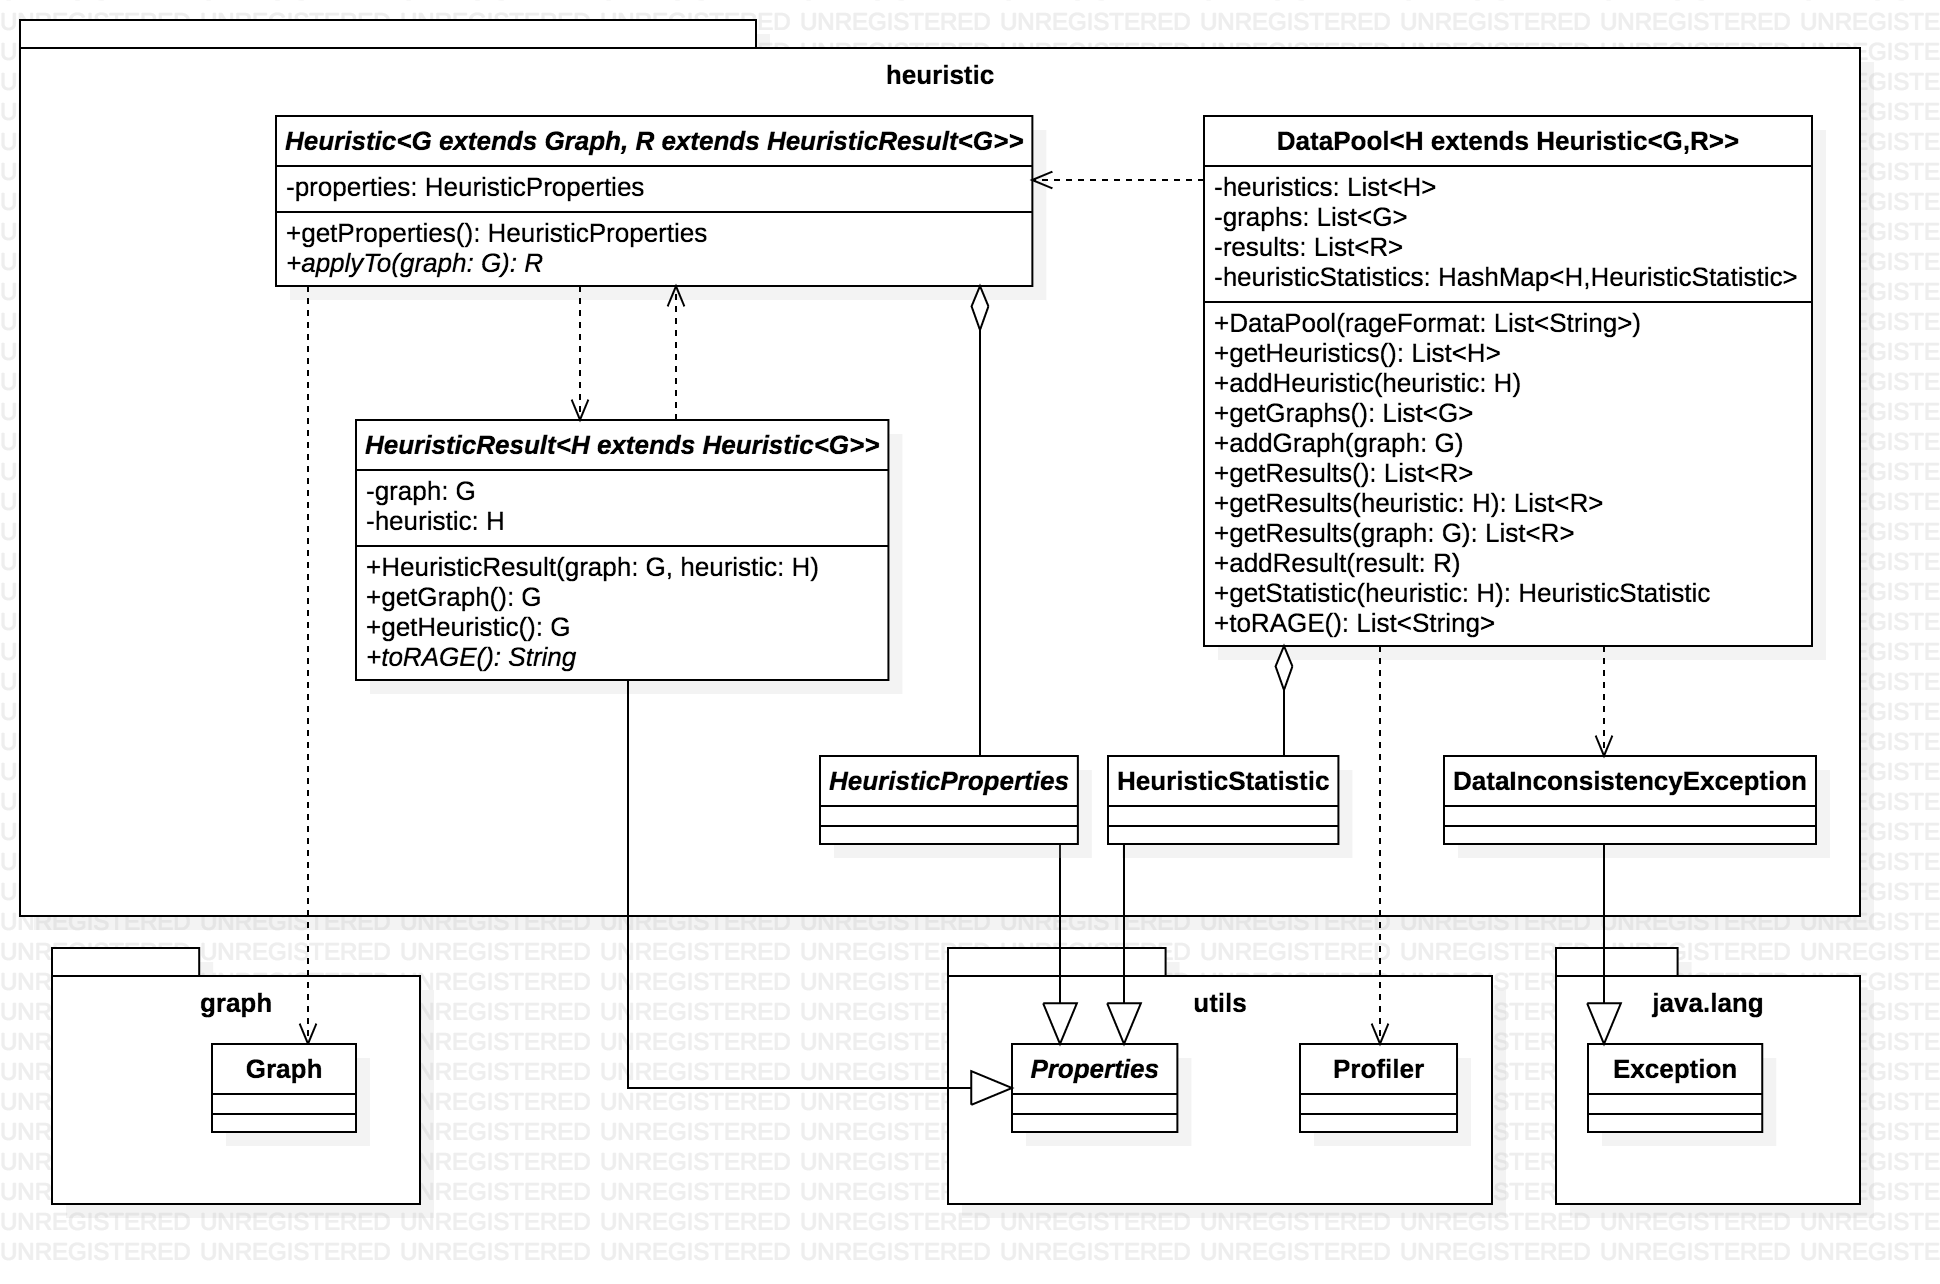
\includegraphics[width=\textwidth]{abbildungen/heuristic.png}

	\caption{Das Paket heuristic }
	\label{img:heuristik}
\end{figure}
	
	\mypackage{heuristic}
	The package contains the interface for implementing heuristics. In the subpackages some heuristics for the total coloring conjecture as well as for the Erdös-Faber-Lovasz conjecture are implemented.
	
	
	
	\myclass{Heuristic}
	
	\textbf{Description}
	
	The class is the abstract interface of a heuristic which is applied to a graph of typ \textbf{G} which has a result of type \textbf{R}.
	
	\textbf{Documentation}
	\begin{enumerate}[+]
		\item{
			\textbf{Heuristic(properties: HeuristicProperties)} \newline
			A constructor for this class \newline
			\textbf{@param properties} the properties defining this heuristic
		}
		\item{
			\textbf{getProperties(): HeuristicProperties} \newline
			\textbf{@return} returns the properties of this heuristic
		}
		\item{
			\textbf{\textit{applyTo(graph: G): R}} \newline
			\textbf{@param graph} the graph of type \textbf{G} on which the heuristic will be applied \newline
			\textbf{@return} returns the result of the heuristic application
		}
	\end{enumerate}
	
	~\newline
	~\newline
	~\newline
	
	\myclass{HeuristicResult}
	
	\textbf{Description}
	
	This class is the abstract interface of the result of a specific calculation of an heuristic \textbf{H} on a specific graph of type \textbf{G}. 
	
	\textbf{Documentation}
	\begin{enumerate}[+]
		\item{
			\textbf{HeuristicResult(graph: G, heuristic: H)} \newline
			The constructor of this class \newline
			\textbf{@param graph} the graph this heuristic was calculated upon \newline
			\textbf{@param heuristic} the heuristic by which the result was calculated
		}
		\item{
			\textbf{getGraph(): G} \newline
			\textbf{@return} returns the graph this result was calculated upon
		}
		\item{
			\textbf{getHeuristic(): H} \newline
			\textbf{@return} returns the heuristic by which this result was calculated
		}
		\item{
			\textbf{\textit{toRAGE(): List<String>}} \newline
			\textbf{@return} returns the line-by-line representation of this heuristic result as specified in the RAGE data format
		}
	\end{enumerate}
	
	~\newpage
	
	\myclass{HeuristicProperties}
	
	\textbf{Description}
	
	This class serves as collection of data for exchange between controller and model, especially to transfer properties of heuristics. It assures that the following properties may be retrieved and set at any time:
	
	\begin{enumerate}[--]
		\item{''name'' -- ein String}
		\item{"valid" -- ein Boolean}
	\end{enumerate}
	
	~\newline
	~\newline
	~\newline
	
	\myclass{DataPool}
	\textbf{Description}
	
	The class manages the application of heuristics of type \textbf{H} on graphs of type \textbf{G} which results have type \textbf{R}. It assures that every heuristic stored in the pool is applied to every graph stored in the pool. Moreover it gathers statistics over this applications.
	
	\textbf{Documentation}
	\begin{enumerate}[+]
		\item{
			\textbf{DataPool(rageFormat: List<String>)} \newline
			A constructor for this class, assuring that the datapool can be loaded from harddrive \newline
			\textbf{@param rageFormat} the line by line representation of a datapool as specified in the RAGE data format.
		}
		\item{
			\textbf{getHeuristics(): List<H>} \newline
			\textbf{@return} returns the list of heuristics currently in this data pool
		}
		\item{
			\textbf{addHeuristic(heuristic: H)} \newline
			\textbf{@param heuristic} the heuristic to be added to data pool, which then will be applied to every graph in the data pool \newline
			\textbf{@throws DataInconsistencyException} if heuristic may not be applied on graphs of type \textbf{G} or does not has results of type \textbf{R}
		}
		\item{
			\textbf{getGraphs(): List<G>} \newline
			\textbf{@return} returns the list of graphs currently in this data pool
		}
		\item{
			\textbf{addGraph(graph: G)} \newline
			\textbf{@param graph} the graph to be added to the data pool, on which then all heuristics in the data pool will be applied \newline
			\textbf{@throws DataInconsistencyException} if heuristics of type \textbf{H} may not be applied on this graph
		}
		\item{
			\textbf{getResults(): List<R>} \newline
			\textbf{@return} returns the list of all results calculated on graphs by heuristics in this data pool
		}
		\item{
			\textbf{getResults(heuristic: H): List<R>} \newline
			\textbf{@param heuristic} the heuristic the results were calculated by \newline
			\textbf{@return} returns all results calculated by \textbf{heuristic} on graphs in this data pool 
		}
		\item{
			\textbf{getResults(graph: G)} \newline
			\textbf{@param graph} the graph the results were calculated upon \newline
			\textbf{@return} returns all results calculated on \textbf{graph} by heuristics in this data pool
		}
		~\newpage
		\item{
			\textbf{getStatistics(heuristic: H): HeuristicStatistic} \newline
			\textbf{@param heuristic} the heuristic whose statistics are requested \newline
			\textbf{@return} returns the statistic gathered for \textbf{heuristic} \newline
			\textbf{@throws DataInconsistencyException} if \textbf{heuristic} is not a heuristic of this data pool
		}
		\item{
			\textbf{toRAGE(): List<String>} \newline
			\textbf{@return} returns the line by line representation of this data pool as specified in the RAGE data format
		}
	\end{enumerate}
	
	~\newline
	~\newline
	~\newline
	
	\myclass{HeuristicStatistic}
	
	This class collects some statistics overt the applications of a specific heuristic within a data pool. It assures that the following properties may be retrieved at any time:
	
	\begin{enumerate}[--]
		\item{''minRuntime'' -- a floating point number}
		\item{''avgRuntime'' -- a floating point number}
		\item{"maxRuntime" -- a floating point number}
		\item{"numApplications" -- a nonnegative integer}
		\item{"numSuccesses" -- a nonnegative integer}
	\end{enumerate}
	
	~\newline
	~\newline
	~\newline
	
	\myclass{DataInconsistencyException}
	
	\textbf{Description}
	
	This class extends the usual Java Exception to an exception specifically thrown when data pools are treated wrong.
	
	~\newpage
	
	
	
	
	
	\mypackage{heuristic.totalColoring}
	In this package and its subpackages some heuristics for the \textbf{total coloring conjecture} (ie. any simple undirected graph with maximal degree $\Delta$ has a total coloring with $\Delta + 2$ colors) are implemented.
	
	
	%TODO tc.png UML
		\begin{figure}
	\centering
	%\fbox{	
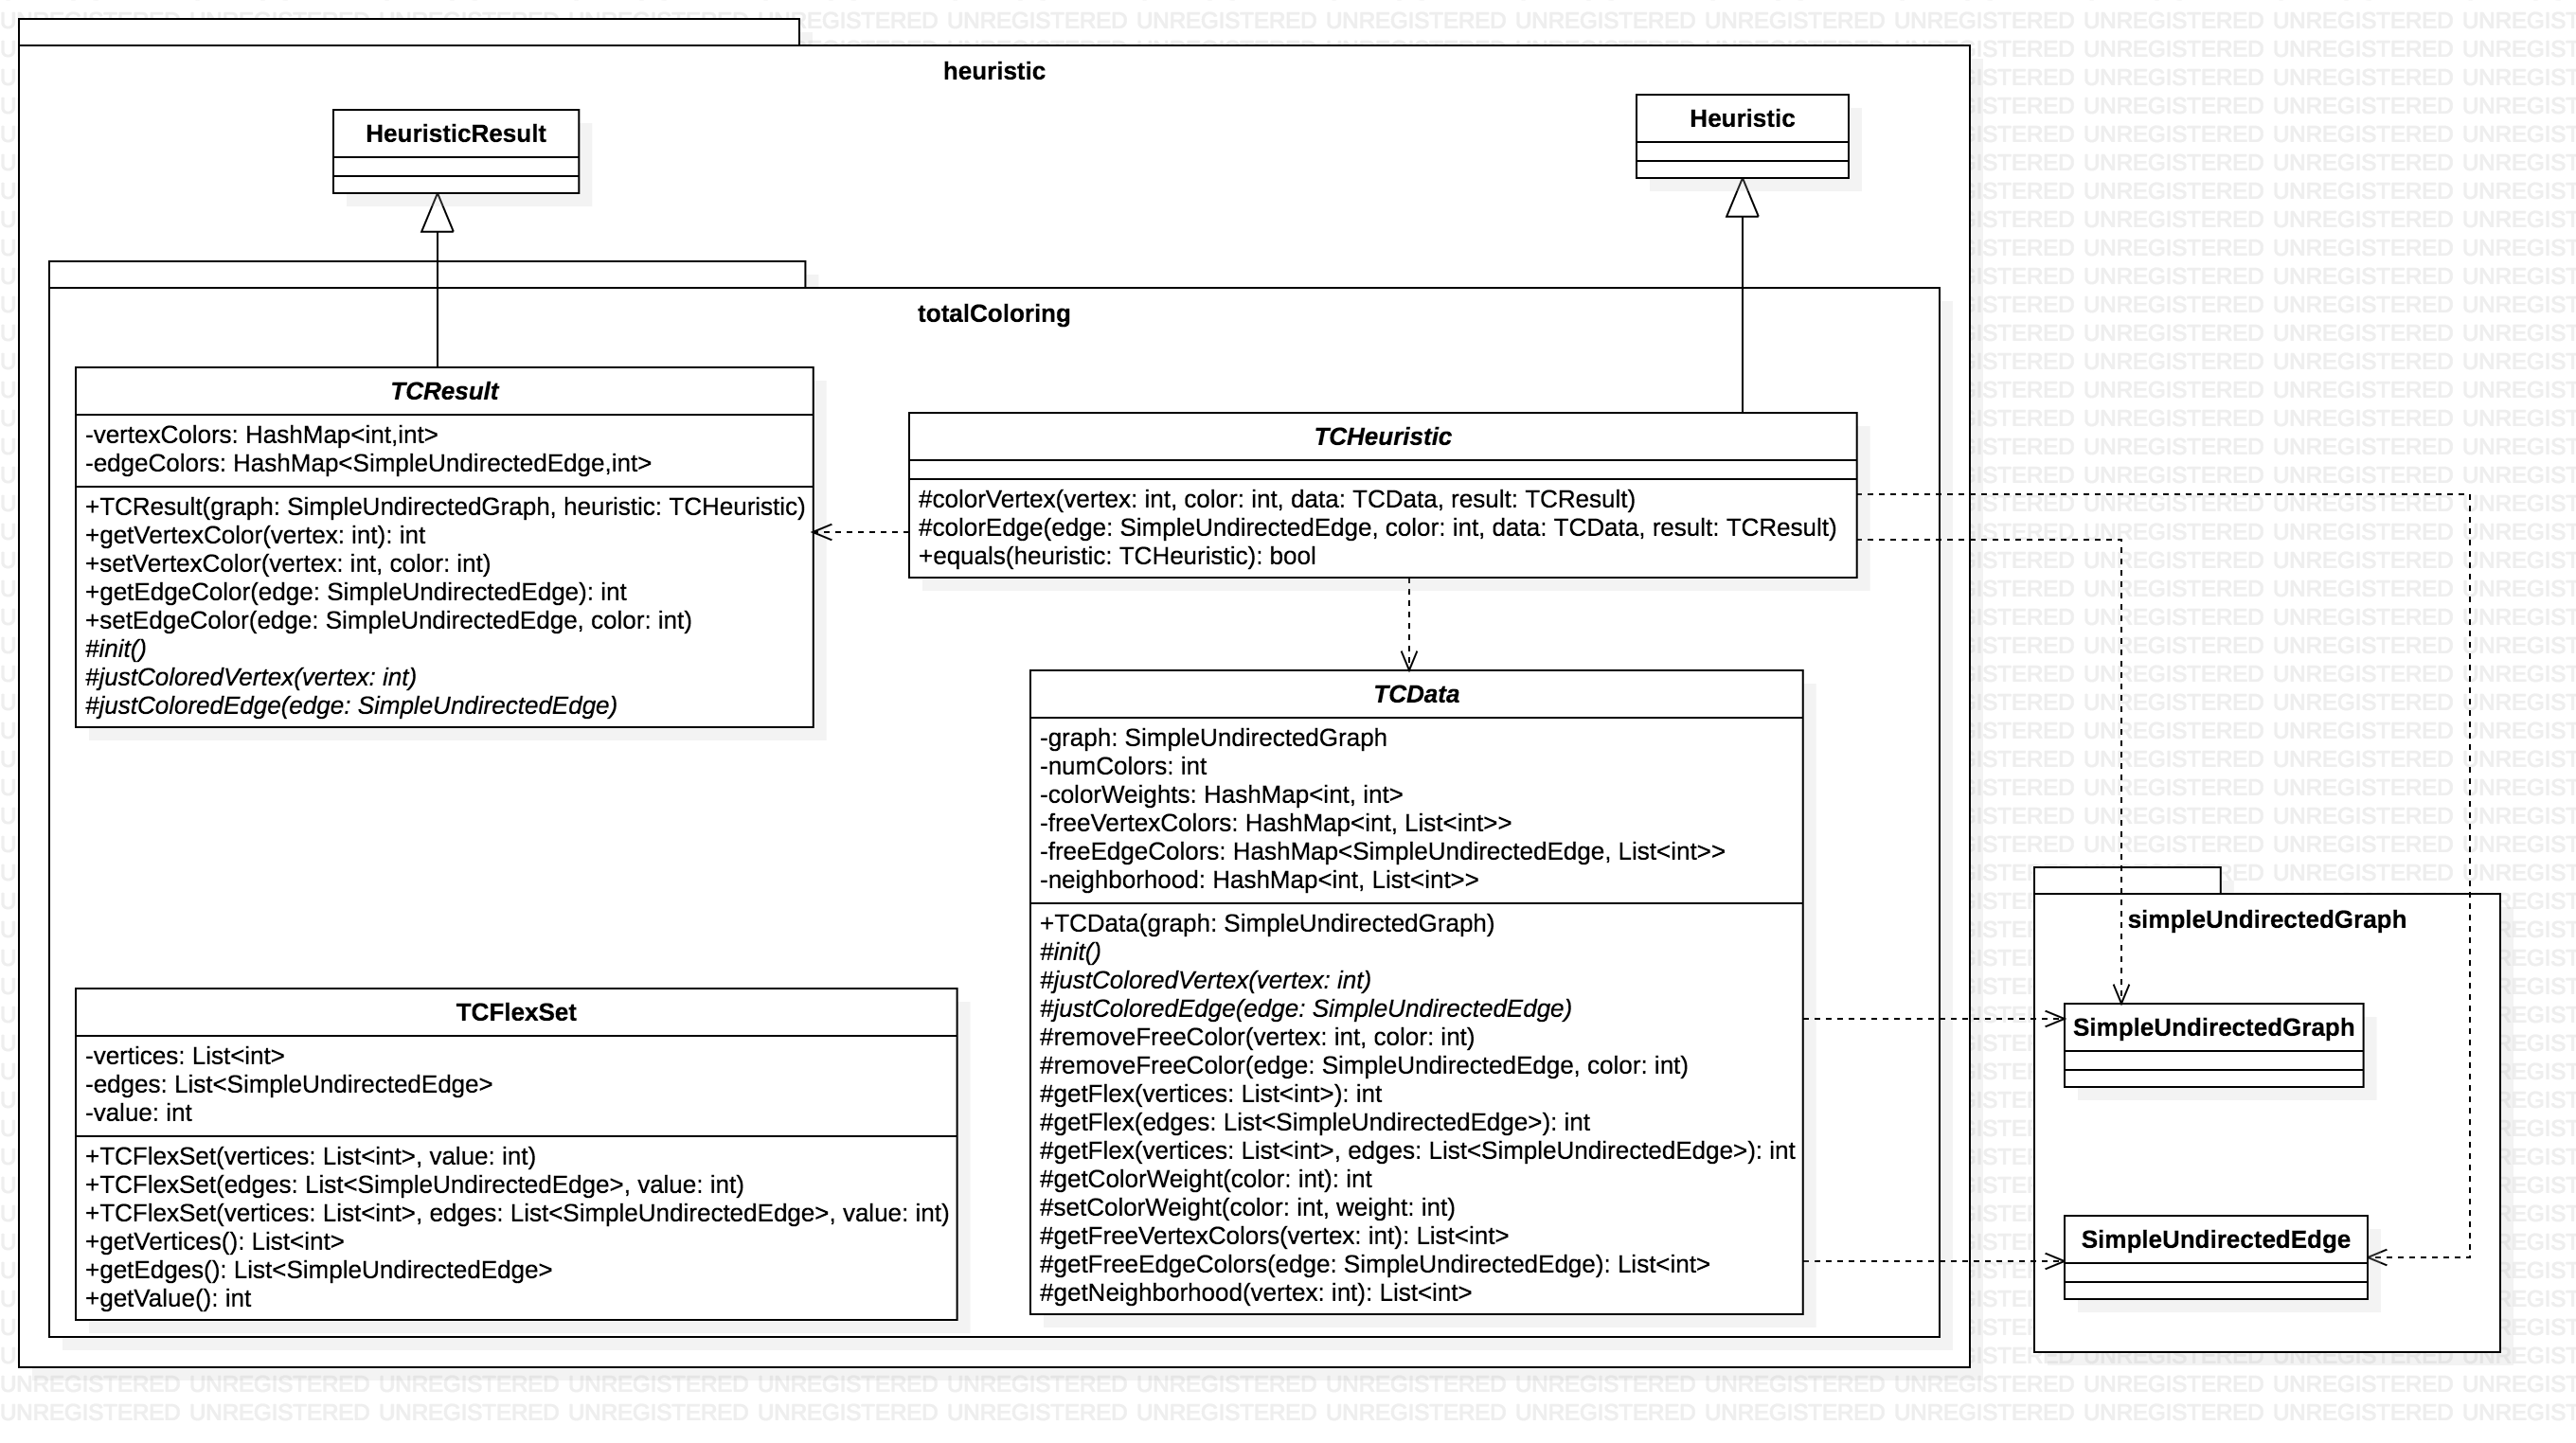
\includegraphics[width=\textwidth]{abbildungen/tc.png}

	\caption{ totalColoring}
	\label{img:tc}
\end{figure}
	
	\myclass{TCHeuristic}
	
	\textbf{Description}
	
	This abstract class is the abstract interface for a total coloring heuristic. It assures that any total coloring heuristic is calculated on SimpleUndirectedGraphs and returns a TCResult as result. It provides some methods, which any total coloring heuristic needs, such as coloring vertices and edges.
	
	\textbf{Documentation}
	\begin{enumerate}[+]
		\item[\#]{
			\textbf{colorVertex(vertex: int, color: int, data: TCData, result: TCResult)} \newline
			\textbf{@param vertex} the vertex to be colored \newline
			\textbf{@param color} the color which will be assigned to the vertex \newline
			\textbf{@param data} the data required for the calculation of a total coloring \newline
			\textbf{@param result} the resulting total coloring
		}
		\item[\#]{
			\textbf{colorEdge(edge: SimpleUndirectedEdge, color: int, data: TCData, result: TCResult)} \newline
			\textbf{@param edge} the edge to be colored \newline
			\textbf{@param color} the color which will be assigned to the edge \newline
			\textbf{@param data} the data required for the calculation of a total coloring \newline
			\textbf{@param result} the resulting total coloring
		}
		\item{
			\textbf{equals(heuristic: TCHeuristic): bool} \newline
			\textbf{@param heuristic} another TCHeuristic this will be compared to \newline
			\textbf{@return} returns \textbf{true} iff the other TCHeuristic of of the same type and has exactly the same properties
		}
	\end{enumerate}
	
	~\newline
	~\newline
	~\newline
	
	\myclass{TCResult}
	
	\textbf{Description}
	
	This class represents a total coloring of a simple undirected graph ie. a coloring of vertices and edges, such that no two adjacent or incident objects share the same color. Colors are represented as integers.
	
	\textbf{Documentation}
	\begin{enumerate}[+]
		\item{
			\textbf{TCResult(graph: SimpleUndirectedGraph, heuristic: TCHeuristic)} \newline
			A constructor for this class
			\textbf{@param graph} the graph this result was calculated upon \newline
			\textbf{@param heuristic} the heuristic this result was calculated by
		}
		\item{
			\textbf{getVertexColor(vertex: int): int} \newline
			\textbf{@param vertex} the vertex whose color is requested \newline
			\textbf{@return} returns the color of \textbf{vertex} \newline
			\textbf{@throws DataInconsistencyException} if vertex has no color
		}
		\item{
			\textbf{setVertexColor(vertex: int, color: int)} \newline
			\textbf{@param vertex} the vertex to be colored \newline
			\textbf{@param color} the color to color \textbf{vertex} with
		}
		\item{
			\textbf{getEdgeColor(edge: SimpleUndirectedEdge): int} \newline
			\textbf{@param edge} the edge whose color is requested \newline
			\textbf{@return} returns the color of \textbf{edge} \newline
			\textbf{@throws DataInconsistencyException} if edge has no color
		}
		\item{
			\textbf{setEdgeColor(edge: SimpleUndirectedEdge, color: int)} \newline
			\textbf{@param edge} the edge to be colored \newline
			\textbf{@param color} the color to color \textbf{edge} with
		}
	\end{enumerate}
	
	~\newline
	~\newline
	~\newline
	
	\myclass{TCData}
	
	\textbf{Description}
	
	This abstract class encapsulates the data required temporarly to calculate a total coloring, such as the lists of \textbf{free colors} of uncolored vertices and edges (ie. the colors which are not used by other objects adjacent / incident to them). Moreover it stores the weighted (vertex vs. edges) sum of how often colors are used.
	
	\textbf{Documentation}
	
	\begin{enumerate}[\#]
		\item{
			\textbf{TCData(graph: SimpleUndirectedGraph)} \newline
			A constructor of this class \newline
			\textbf{@param graph} the graph the heuristic is running at
		}
		\item{
			\textbf{\textit{init()}} \newline
			May be implemented to (re-)initialize the data at any time within the running heuristic
		}
		\item{
			\textbf{\textit{justColoredVertex(vertex: int)}} \newline
			May be implemented to update data anytime when a vertex was colored \newline
			\textbf{@param vertex} the vertex which was just colored
		}
		\item{
			\textbf{\textit{justColoredEdge(edge: SimpleUndirectedEdge)}} \newline
			May be implemented to update data anytime when an edge was colored \newline
			\textbf{@param edge} the edge which was just colored
		}
		\item{
			\textbf{removeFreeColor(vertex: int, color: int)} \newline
			\textbf{@param vertex} the vertex which will have one free color less \newline
			\textbf{@param color} the color which \textbf{vertex} mustnt use
		}
		\item{
			\textbf{removeFreeColor(edge: SimpleUndirectedEdge, color: int)} \newline
			\textbf{@param edge} the edge which will have one free color less \newline
			\textbf{@param color} the color which \textbf{edge} mustnt use
		}
		\item{
			\textbf{getFlex(vertices: List<int>): int} \newline
			\textbf{@param vertices} the set of vertices whose flexibility should be calculated \newline
			\textbf{@return} returns the flexibility of these vertices ie. \# of colors free for all vertices -- \# of \textbf{vertices}
		}
		\item{
			\textbf{getFlex(edges: List<SimpleUndirectedEdge>): int} \newline
			\textbf{@param vertices} the set of vertices whose flexibility should be calculated \newline
			\textbf{@return} returns the flexibility of these vertices ie. \# of colors which are free for all edges -- \# of \textbf{edges}
		}
		\item{
			\textbf{getFlex(vertices: List<int>, edges: List<SimpleUndirectedEdge>): int} \newline
			\textbf{@param vertices} a set of vertices \newline
			\textbf{@param edges} a set of edges \newline
			\textbf{@return} returns the flexibility of these objects ie. \# of colors which are free for all objects -- \# of \textbf{objects}
		}
		\item{
			\textbf{getColorWeight(color: int): int} \newline
			\textbf{@param color} the color whose weight is requested \newline
			\textbf{@return} returns the weight of this color ie. how often it was used weighted differently by vertices and edges
		}
		\item{
			\textbf{setColorWeight(color: int, weight: int)} \newline
			\textbf{@param color} the color whose weight will be updated \newline
			\textbf{@param weight} the new weight of \textbf{color}
		}
		\item{
			\textbf{getFreeVertexColors(vertex: int): List<int>} \newline
			\textbf{@param vertex} the vertex whose free colors are requested \newline
			\textbf{@return} returns the list of free colors of \textbf{vertex}
		}
		\item{
			\textbf{getFreeVertexColors(edge: SimpleUndirectedEdge): List<int>} \newline
			\textbf{@param edge} the edge whose free colors are requested \newline
			\textbf{@return} returns the list of free colors of \textbf{edge}
		}
	\end{enumerate}
	
	
	~\newline
	~\newline
	~\newline
	
	\myclass{TCFlexSet}
	
	\textbf{Description}
	
	This class represents a subset of vertices and edges of a graph with a given \textbf{flexibility value} (ie. \# colors free for all objects -- \# objects) used heavily in some TCHeuristics.
	
	\textbf{Documentation}
	\begin{enumerate}[\#]
		\item{
			\textbf{TCFlexSet(vertices: List<int>, value: int)} \newline
			A constructor of this class \newline
			\textbf{@param vertices} some vertices \newline
			\textbf{@param value} the flexibility value of \textbf{vertices}
		}
		\item{
			\textbf{TCFlexSet(edges: List<SimpleUndirectedEdge>, value: int)} \newline
			A constructor of this class \newline
			\textbf{@param edges} some edges \newline
			\textbf{@param value} the flexibility value of \textbf{edges}
		}
		\item{
			\textbf{TCFlexSet(vertices: List<int>, edges: List<SimpleUndirectedEdge>, value: int)} \newline
			A constructor of this class \newline
			\textbf{@param vertices} some vertices \newline
			\textbf{@param edges} some edges \newline
			\textbf{@param value} the flexibility value of the set of objects in \textbf{vertices} and \textbf{edges}
		}
		\item{
			\textbf{getVertices(): List<int>} \newline
			\textbf{@return} returns the vertices in this flex set
		}
		\item{
			\textbf{getEdges(): List<SimpleUndirectedEdge>} \newline
			\textbf{@return} returns the edges in this flex set
		}
		\item{
			\textbf{getValue(): int} \newline
			\textbf{@return} returns the flexibility value of this set of objects
		}
	\end{enumerate}
	
	~\newpage
	
	
	
	
	\mypackage{heuristic.totalColoring.greedy}
	In this package some greedy heuristics for the total coloring conjecture are implemented. They all have in common, that the vertices are colored first and the edges are colored afterwards. The heuristics differ in the way the edges are colored.
	
	\myclass{TCGreedyData}
	
	\textbf{Description}
	
	Since TCData is abstract this class is required such that the TCGreedy heuristic has its own data class, even if with respect to TCData no additional attributes or methods are added.
	
	\myclass{TCGreedy}
	
	\textbf{Description}
	
	This class implements the TCGreedy heuristic which tries to calculate a total coloring.
	
	\textbf{Documentation}
	\begin{enumerate}[+]
		\item{
			\textbf{applyTo(graph: SimpleUndirectedGraph): TCResult} \newline
			implements the following heuristic
			
			\begin{verbatim}
				for every vertex v in order of a breadth first search
				    if v cannot be colored
				        return incomplete coloring
				    get minimally used free color c of v with respect to the color weights
				    color v with color c
				    
				for every vertex v in order of a breadth first search
				    for every uncolored edge e incident to v in the order defined on edges
				        if e cannot be colored
				            return incomplete coloring
				        get minimally used free color c of e with respect to the color weights
				        color e with color c
				        
				return complete coloring
			\end{verbatim}
			
			\textbf{@param graph} the graph this heuristic will be applied on \newline
			\textbf{@return} returns the calculated coloring
		}
	\end{enumerate}
	
	~\newpage
	
	\myclass{TCGreedyOneData}
	
	\textbf{Description}
	
	This class stores all uncolored edges with exactly one free color temporarily.
	
	\textbf{Documentation}
	
	\begin{enumerate}[\#]
		\item{
			\textbf{init()} \newline
			initializes the list of all uncolored edges with exactly one free color
		}
		\item{
			\textbf{justColoredEdge(edge: SimpleUndirectedEdge)} \newline
			updates the list of edges with exactly one free color \newline
			\textbf{@param edge} the edge which was just colored
		}
		\item[-]{
			\textbf{calcSingularEdges()} \newline
			updates the list of edges with exactly one free color
		}
		\item{
			\textbf{getMinimalSingularEdge(): SimpleUndirectedEdge} \newline
			\textbf{@return} returns the minimal edge with exactly one free color with respect to the order defined on edges
		}
	\end{enumerate}
	
	\myclass{TCGreedyOne}
	
	\textbf{Description}
	
	This class implements the TCGreedyOne heuristic which tries to calculate a total coloring.
	
	\textbf{Documentation}
	
	\begin{enumerate}[+]
		\item{
			\textbf{applyTo(graph: SimpleUndirectedGraph): TCResult} \newline
			implements the following heuristic
			
			\begin{verbatim}
				for every vertex v in the order of a breadth first search
				    if v cannot be colored
				        return incomplete coloring
				    get minimally used free color c of v with respect to the color weights
				    color v with color c
				    
				for every vertex v in the order of a breadth first search
				    for every uncolored edge e incident to v in the order defined on edges
				        while there are uncolored edges with exactly one free color
				            get minimal uncolored edge with exactly one free color f
				            get minimally used free color c of f with respect to the color weights
				            color f with color c
				        if e is colored already
				            continue
				        if e cannot be colored
				            return incomplete coloring
				        get minimally used free color c of e with respect to the color weights
				        color e with color c
				        
				return complete coloring
			\end{verbatim}
			
			\textbf{@param graph} the graph this heuristic will be calculated on \newline
			\textbf{@return} returns the calculated coloring
		}
	\end{enumerate}
	
	~\newpage
	
	\myclass{TCGreedyFewData}
	
	\textbf{Description}
	
	This class stores all uncolored edges sorted first by their amount of free colors and then by the order defined on edges.
	
	\textbf{Documentation}
	
	\begin{enumerate}[\#]
		\item{
			\textbf{init()} \newline
			initializes the list of uncolored edges
		}
		\item{
			\textbf{justColoredEdge(edge: SimpleUndirectedEdge)} \newline
			updates the list of uncolored edges
		}
		\item{
			\textbf{getMinimalUncoloredEdge(): SimpleUndirectedEdge} \newline
			\textbf{@return} returns the minimal uncolored edge with respect to the number of free colors and the order defined on edges
		}
	\end{enumerate}
	
	\myclass{TCGreedyFew}
	
	\textbf{Description}
	
	This class implements the TCGreedyFew heuristic, which tries to calculate a total coloring.
	
	\textbf{Documentation}
	
	\begin{enumerate}[+]
		\item{
			\textbf{applyTo(graph: SimpleUndirectedGraph): TCResult} \newline
			implements the following heuristic
			
			\begin{verbatim}
				for every vertex v in the order of a breadth first search
				    if v cannot be colored
				        return incomplete coloring
				    get minimally used free color c of v with respect to the color weights
				    color v with color c
				    
				for every vertex v in the order of a breadth first search
				    for every uncolored edge e incident to v in the order defined on edges
				        while there are uncolored edges with less free colors than e and lower order than e
				            get minimal uncolored edge f
				            if f cannot be colored
				                return incomplete coloring
				            get minimally used free color c of f with respect to the color weights
				            color f with color c
				        if e is colored already
				            continue
				        if e cannot be colored
				            return incomplete coloring
				        get minimally used free color c of e with respect to the color weights
				        color e with color c
				        
				return complete coloring
			\end{verbatim}
			
			\textbf{@param graph} the graph this heuristic will be calculated on \newline
			\textbf{@return} returns the calculated coloring
		}
	\end{enumerate}
	
	~\newpage
	
	\myclass{TCGreedySetData}
	
	\textbf{Description}
	
	This class stores for any vertex v the subset of all uncolored edges incident to v which has the lowest flexibility value (ie. \# of colors which are free for every edge in this set -- \# of edges in the set) and is the lowest with respect to lexicographic ordering using the order defined on edges. These sets are from now on referred to as minimal flex sets
		
	\textbf{Documentation}
	
	\begin{enumerate}[\#]
		\item{
			\textbf{init()} \newline
			initializes the minimal flex sets
		}
		\item{
			\textbf{justColoredEdge(edge: SimpleUndirectedEdge)} \newline
			updates the minimal flex sets of the vertices incident to edge
		}
		\item[-]{
			\textbf{calcMinimalFlexSet(vertex: int)} \newline
			calculates the minimal flex set of \textbf{vertex} \newline
			\textbf{@param vertex} the vertex whose minimal flex set is calculated
		}
		\item{
			\textbf{getMinimalFlexSet(): TCFlexSet} \newline
			\textbf{@return} returns the minimal flex set belonging to the vertex with minimal index
		}
	\end{enumerate}
	
	\myclass{TCGreedySet}
	
	\textbf{Description}
	
	This class implements the TCGreedySet heuristic, which tries to calculate a total coloring.
	
	\textbf{Documentation}
			
	
	\begin{enumerate}[+]
		\item 
			\textbf{applyTo(graph: SimpleUndirectedGraph): TCResult} \newline
			implements the following heuristic		
		%[numbers=left,resetmargins=true,frame=single,commandchars=\\\{\}]		
						
			\begin{verbatim}
				for every vertex v in the order of a breadth first search
				    if v cannot be colored
				        return incomplete coloring
				    get minimally used free color c of v with respect to the color weights
				    color v with color c
				    
				while there is a set with minimal flexibility
				    find the set X of minimal flexibility belonging to the vertex v with lowest index
				        if X has negative flexibility
				            return incomplete coloring
				        for every edge e of X in the order defined on edges
				            if e cannot be colored
				                return incomplete coloring
				            get minimally used free color c of e with respect to the color weights
				            color e with color c
				        
				return complete coloring			
			\end{verbatim}
			
			
			\textbf{@param graph} the graph this heuristic will be calculated on \newline
			\textbf{@return} returns the calculated coloring
		
	\end{enumerate}
	
	~\newpage
	
	\myclass{TCGreedyConData}
	
	\textbf{Description}
	
	This class stores the list of uncolored edges temporarily to compute connected subsets of uncolored edges up to a specific size.
		
	\textbf{Documentation}
	
	\begin{enumerate}[\#]
		\item{
			\textbf{init()} \newline
			initializes the list of uncolored edges
		}
		\item{
			\textbf{justColoredEdge(edge: SimpleUndirectedEdge)} \newline
			updates the list of uncolored edges
		}
		\item{
			\textbf{getMinimalFlexSet(): TCFlexSet} \newline
			\textbf{@return} returns the connected set of uncolored edges with minimal flexibility value (\# of colors which are free for all edges -- \# of edges) and minimal lexicographic order using the order defined on edges.
		}
	\end{enumerate}
	
	\myclass{TCGreedyCon}
	
	This class implements the TCGreedyCon heuristic, which tries to calculate a total coloring.
	
	\textbf{Documentation}
	
	\begin{enumerate}[+]
		\item{
			\textbf{applyTo(graph: SimpleUndirectedGraph): TCResult} \newline
			implements the following heuristic
			
			\begin{verbatim}
				for every vertex v in the order of a breadth first search
				    if v cannot be colored
				        return incomplete coloring
				    get minimally used free color c of v with respect to the color weights
				    color v with color c
				    
				while there is a set with minimal flexibility
				    find the set X of minimal flexibility which has the lowest lexicographic order
				        if X has negative flexibility
				            return incomplete coloring
				        for every edge e of X in the order defined on edges
				            if e cannot be colored
				                return incomplete coloring
				            get minimally used free color c of e with respect to the color weights
				            color e with color c
				        
				return complete coloring
			\end{verbatim}
			
			\textbf{@param graph} the graph this heuristic will be calculated on \newline
			\textbf{@return} returns the calculated coloring
		}
	\end{enumerate}
	
	
	
	
	
	\mypackage{heuristic.totalColoring.mixedGreedy}
	In this package some heuristics for the total coloring conjecture are implemented. In comparison to the greedy heuristics, these heuristics do not seperate the coloring of vertices and edges strictly but rather alternate between them.
	
	
	\myclass{TCMixedGreedyData}
	\myclass{TCMixedGreedy}
	
	~\newpage
	
	\myclass{TCMixedGreedyOneData}
	\myclass{TCMixedGreedyOne}
	
	~\newpage
	
	\myclass{TCMixedGreedyFewData}
	\myclass{TCMixedGreedyFew}
	
	~\newpage
	
	\myclass{TCMixedGreedySetData}
	\myclass{TCMixedGreedySet}
	
	~\newpage
	
	\myclass{TCMixedGreedyConData}
	\myclass{TCMixedGreedyCon}
	
	
	
	
	
	\mypackage{heuristic.erdosFaberLovasz}
	\myclass{EFLHeuristic}
	\myclass{EFLResult}
	
	\mypackage{heuristic.erdosFaberLovasz.greedy}
	\myclass{EFLGreedyData}
	\myclass{EFLGreedy}
	\myclass{EFLGreedyOneData}
	\myclass{EFLGreedyOne}
	\myclass{EFLGreedyFewData}
	\myclass{EFLGreedyFew}
	\myclass{EFLGreedySetData}
	\myclass{EFLGreedySet}
	\myclass{EFLGreedyConData}
	\myclass{EFLGreedyCon}
	
	
	\section{View}
		%\begin{enumerate}
	\subsection{Allgemein}
		%Einleitung
		Kommen wir nun zum nächsten Großen Abschnitt des Programm-Entwurfs.
		Nachdem wir im letzten Abschnitt über das Model gesprochen haben folgt nun der View-Teil des "Model-View-Controller"-Entwurfsmusters.
		Die View beschäftigt sich, wie der Name andeutet mit dem Aussehen des Programms und somit mit der graphischen Repräsentation.
		
		%Überleitung:
		Wie im Pflichtenheft beschreiben haben wir uns für die Entwicklung mit Java entschieden.
		Unter Java gibt es mehrere Möglichkeiten eine GUI zu erstellen.
			
			\begin{enumerate}
				\item Standart Widget Toolkit (SWT)
				\item Abstract Widget Toolkit (AWT)
				\item Swing
				\item JavaFx
			\end{enumerate}

		Uns war allerdings relativ schnell klar, dass die Wahl auf JavaFx fallen wird.
		Dies lag nicht zuletzt an FXML und der bisherigen Entwicklungs-Erfahrung.
		Dazu gleich mehr.
		
			\subsubsection{JavaFX}
			%Allgemeine Beschreibung:
			\begin{itemize}
			\item JavaFX ist eine Abkürzung für Java Graphics.
			\item JavaFX ist eine Möglichkeit unter Java eine graphische Oberfläche zu erstellen.
			\item JavaFX ist eine komplette Neuentwicklung von Oracle.
			\item Es ist unabhängig von den bisherigen Methoden AWT und Swing.
			\item JavaFX wurde 2014 veröffentlicht.
			\item Es ist seit Version 7.6 in x86 Java Standard Edition (JavaSE) Runtime Installation enthalten.
			\item Da wir mit Java 8 arbeiten werden ist dies somit kein Problem.
			\end{itemize}
			
			%Aufbau
			JavaFX arbeitet mit einem Szenengraphen (engl. scene graph), der die einzelnen Bestandteile einer GUI verwaltet.
			Auf diesen werden dann alle weiteren Bestandteile gesetzt.
			
			\subsubsection{FXML}
				%Einleitung:
				Wie auch bei den alternativen kann man natürlich auch mit JavaFx über zu schreibenden Code GUI-Objekte erstellen und diese auf den Scenen-Graphen aufbringen.
				Allerdings besteht mit JavaFx erstmals die Möglichkeit eine neue Form der GUI Entwicklung zu beschreiten.
				Diese erfolgt in Form von FXML.
				
				%Allgemeine Beschreibung:
				FXML ist eine deklarative Beschreibung der grafischen Oberflächen auf XML-Basis.
				Dies bietet einige Vorteile gegenüber der konventionellen GUI-Entwicklung.
				Zum einen ist durch diese Technologie die Trennung des Designs der GUI und deren Funktionalität strikt getrennt.
				Zum anderen ist das Einfügen von GUI-Bestandteilen, die an mehreren Stellen der Benutzeroberfläche zum Einsatz kommen sehr einfach möglich.
				Dies Ermöglicht, dass der mehrfachverwendbare Code nur einmal in einem Separatem FXML-Dokument abgespeichert werden muss und dann über den „include-Tag“ an allen Stellen verwendet werden kann.
				Darüber hinaus können für die Gestaltung auch Web-Technologien wie CSS eingesetzt werden.
				Dies sorgt zusätzlich für eine Trennung von Layout auf der einen und Style und Design auf der anderen Seite, da separate CSS-Dateien erstellt werden können.
				Diese können dann in den FXML-Code eingebettet werden, sodass die GUI das Design übernehmen kann.
				
				%Entwicklung:
				Die Entwicklung der FXML-Dateien erfolgt zuerst über den SceneBuilder.
				Dieser ist ein grafisches Tool, das die Erstellung von FXML-Dateien vereinfacht.
				Der daraus generierte Code wird bei Bedarf dann nochmals per Hand nachbearbeitet.
				Zur Nachbereitung zählen unter anderem auch das Einfügen der „include-Tags“ (wie oben beschrieben).
%			}
	%	}
	
	\subsection{Entwurf}
		%Einführung
		Der Entwurf der View gliedert sich prinzipiell in folgende Pakete auf:
			\begin{enumerate}
				\item Graphic
				\item Drawer
				\item Sound
			\end{enumerate}
		Diese sind Sup-Pakete des "View-Packages" und werden im folgenden genauestens unter die Lupe genommen.

		\mypackage{Graphic}
		The Graphic-Package is a Package for some adaptations and expansions with the JavaFx Stuff.
		
		\mypackage{Graphic.UIElements}
		The UI-Elements-Package contains new created UI-Elements that expand the JavaFx-UI.
		
		\myclass{ZoomableScrollPane}
		
			\textbf{Beschreibung}\newline
			This is an expansion to the JavaFx-ScrollPane.
			This adds the ScrollPane that it can be zoomed.
			
			This is used so that the drawn Graph could be zoomed in/out so that the user can easily look for some Edges.
			
			This Class is not made by ourself.
			@author
			https://www.pixelduke.com/2012/09/16/zooming-inside-a-scrollpane/
			
			\textbf{Dokumentation}\newline
			Because this Class is already fully implemented by the creator, there will be no Documentation from our side.

	\mypackage{Drawer}
	The Drawer-Package.
	This Package contains everything that belongs to the Drawing of the Graphs.
	It is a upper-Package, therefore no further Documentation for this.
	
		\begin{figure}
	\centering
	%\fbox{	
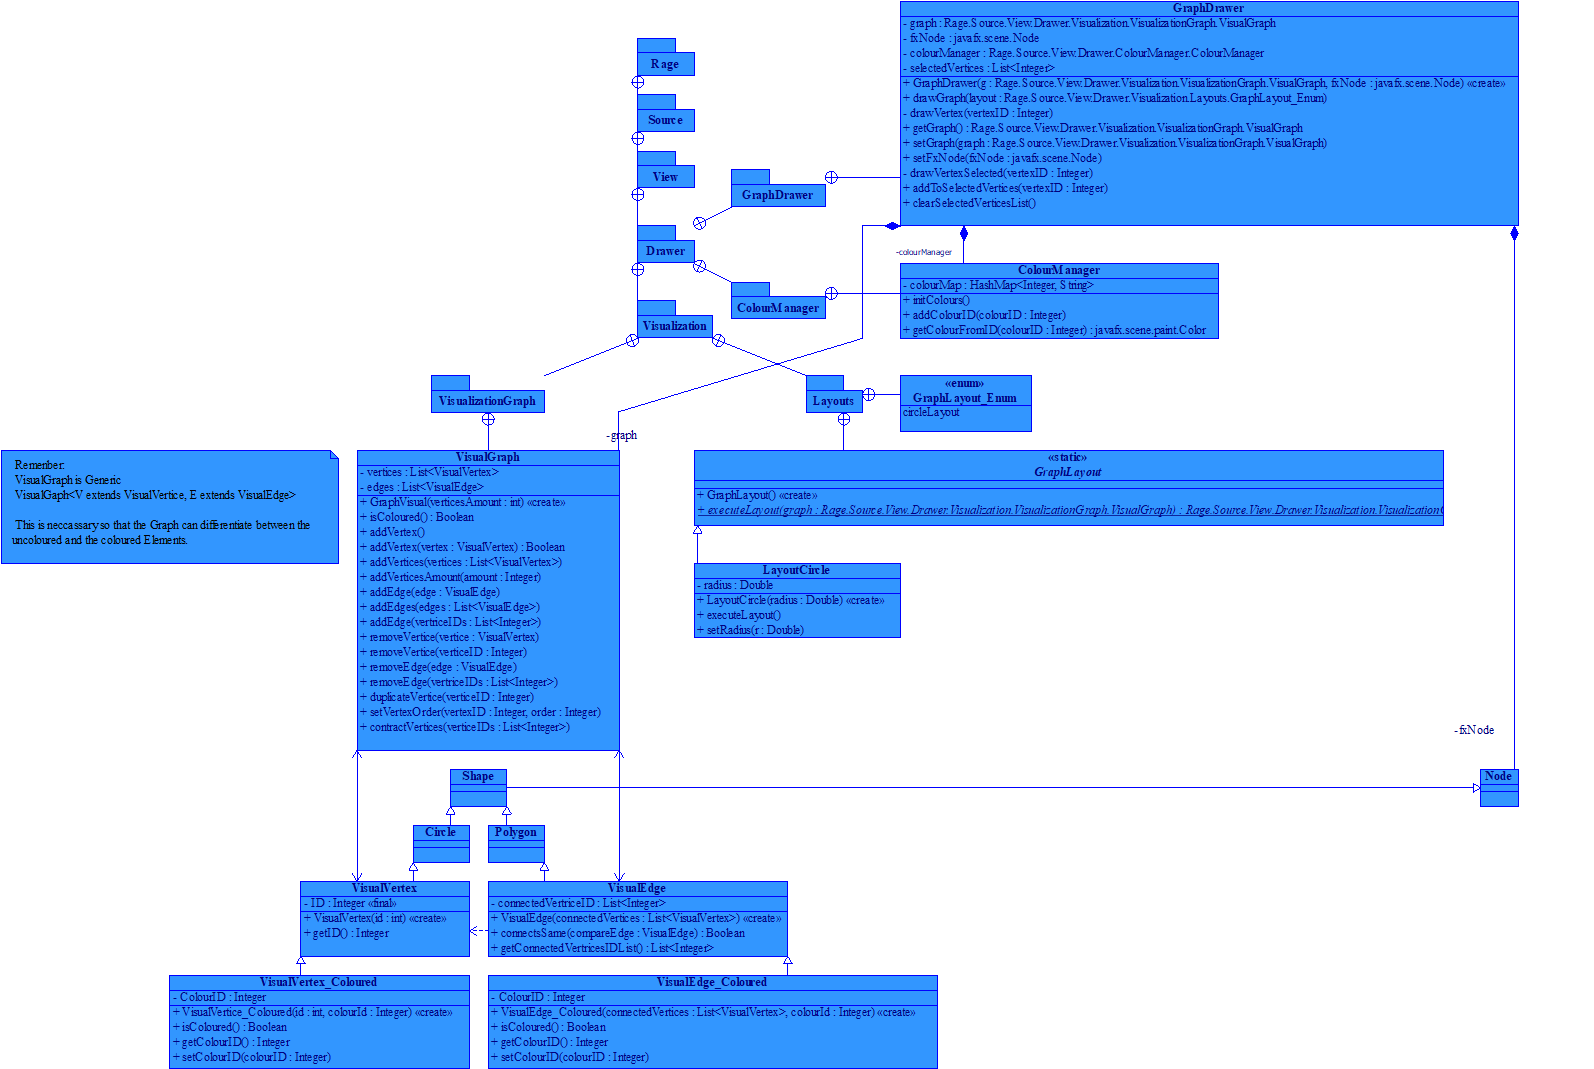
\includegraphics[width=\textwidth]{abbildungen/ClassDiagram_View_Drawer.png}
\caption{ViewDrawer }
	\label{img:viewdrawer}
	\end{figure}
	
	%Hier das ClassDiagram_View_Drawer einfügen.
	
		\mypackage{Drawer.GraphDrawer}
		The GraphDrawer-Package contains like the Name suggested the GraphDrawer that visualizes the Graph and "draws" it to a JavaFx-Node for the User.
		
			\myclass{GraphDrawer}			
				\textbf{Beschreibung}\newline
				The Drawer that draws the given Graph to the given JavaFx-Node.				
				\textbf{Dokumentation}\newline
				\begin{enumerate}[-]
					\item{
						\textbf{graph : VisualGraph} \newline
						The Graph that should be drawn.
					}
					\item{
						\textbf{fxNode : javafx.scene.Node} \newline
						The JavaFx-Node where the Graph should be drawn on.
					}
					\item{
						\textbf{colourManager : ColourManager} \newline
						The ColourManager of this Drawer to Map the ColourID's to the actual Colours of the to drawn Objects.
						
						This Object is created at the Constructor as new ColourManager and before the Drawing the ColourID's are added.
					}
					\item{
						\textbf{selectedVertices : List<Integer>} \newline
						The List of Vertices-ID's that the user selected the Vertices at the GUI.
					}
				\end{enumerate}
				\begin{enumerate}[+]
					\item{
						\textbf{GraphDrawer(graph : VisualGraph, fxNode : javafx.scene.Node)} \newline
						The Constructor of this Class.
						
						Sets the given Graph and fxNode.
						Also initializes the ColourManager.
						\newline
						\textbf{@param graph}
							The Graph that should be set as the Graph of this Drawer.
							\newline
						\textbf{@param fxNode}
							The JavaFx-Node that should be set as the fxNode of this Class.
							\newline
					}
					\item{
						\textbf{printGraphTextual()} \newline
						This Method prints the textual Representation onto the given JavaFx-Node.
						\newline
					}
					\item{
						\textbf{drawGraph(layout : GraphLayoutEnum)} \newline
						This Method draws the Graph to the given JavaFx-Node by using the given Layout to position it's Vertices.
						\newline
						\textbf{@param layout}
							The Enum that indicates which Layout the Drawer should use.
							If it is null the Drawer will use the Circle Layout.
							\newline
					}
					\item[-]{
						\textbf{drawVertex(vertexID : Integer)} \newline
						Draw the given Vertex.
						
						Get the Vertex by searching for the given VertexID at the vertices-List of the given Graph.
						Use the GraphicLayout to get the correct Position of this Vertex.
						\newline
						\textbf{@param vertexID}
							The ID of the to drawn Vertex.
							\newline
					}
					\item[-]{
						\textbf{drawVertexSelected(vertexID : Integer)} \newline
						Draw the given Vertex as a selected Vertex.
						
						This Method is called if the to drawn Vertex of the drawVertex-Method is in the selectedVertices-List.
						
						The Vertex is drawn as selected by adding the corresponding Picture into the Vertex-JavaFx-Shape.
						Then the standard draw-Method is used to do the rest.
						\newline
						\textbf{@param vertexID}
						The ID of the Vertex that should be drawn as a selected Vertex.
						\newline
					}
					\item[-]{
						\textbf{drawEdge(edgePosition : Integer)} \newline
						Draw the Edge that is on the given Position at the Edge-List of the Graph of this Drawer.
						
						This Method only draws one Edge so that the Editor can show specific Edges.
						This Method is also called multiple times to draw all Edges.
						\newline
						\textbf{@param edgePosition}
						The Position of the to drawn Edge at the List of Edges of the Graph.
						\newline
					}
					\item{
						\textbf{addToSelectedVertices(vertexID : Integer)} \newline
						Add the given VertexID to the List of selected ones.
						\newline
						\textbf{@param vertexID}
						The Vertex-ID that should be added to the List of selected Vertices.
						\newline
					}
					\item{
						\textbf{clearSelectedVerticesList()} \newline
						Clear the List of selected Vertices-ID's.
						\newline
					}
					\item{
						\textbf{getGraph() : VisualGraph} \newline
						Get the VisualGraph of this Drawer.
						\newline
						\textbf{@return} returns
							The VisualGraph of this Drawer.
							\newline
					}
					\item{
						\textbf{setGraph(graph : VisualGraph)} \newline
						Set the VisualGraph of this Drawer.
						\newline
						\textbf{@param graph}
							The VisualGraph that should be set.
							\newline
					}
					\item{
						\textbf{setFxNode(fxNode : javafx.scene.Node)} \newline
						Set the JavaFx-Node where the Graph should be drawn on.
						\newline
						\textbf{@param fxNode}
						The  Node that should be set as the JavaFx-Node to draw on.
						\newline
					}
				\end{enumerate}
	
		\mypackage{Drawer.ColourManager}
		The ColourManager-Package.
		This Package only contains the ColourManager which maps the abstract ColourID's that are given by the calculation into a real Colour-Value that could be drawn.
		This Class is separately because it provides a relatively general task, that easily can be (re)used elsewhere.
		
			\myclass{ColourManager}
				\textbf{Beschreibung}\newline
				The ColourManager manages the different Colours by Mapping the ColourID's to an actual Colour-Value, so that the Drawer can draw the coloured Graph by these ColourID's.
				\textbf{Dokumentation}\newline
				\begin{enumerate}[-]
					\item{
						\textbf{colourMap : Hashmap<IntegerString>} \newline
						The HashMap of every ColourID to the actual Colour-Value that is represented as a String.
					}
				\end{enumerate}
				\begin{enumerate}[+]
					\item{
						\textbf{ColourManager()} \newline
						The Empty-Constructor of this Class.
						The Colours are added step by step at a later point.
						\newline
					}
					\item{
						\textbf{ColourManager(colourIDs : List<Integer>)} \newline
						The Constructor of this Class.
						It adds the given ColourID's of the List and puts them into the Hashmap.
						Then the initColours-Method is called so that the mapping is completed for the given ColourId's.
						\newline
						\textbf{@param colourIDs}
							The List of colourID's that should be mapped to real Colour-Values.
							\newline
					}
					\item{
						\textbf{initColours()} \newline
						This Method has to be called when every ColourID is put into the HashMap.
						Then this Method calculates a Assignment of real Colours to the ColourID's and writes them into the HashMap, where it can be read out at a later Time.
						\newline
					}
					\item{
						\textbf{addColourID(colourIDs : Integer)} \newline
						Add a new ColourID to the HashMap, where later the real Colour is mapped to.
						
						It is checked if the given ColourID is already at the HashMap.
						\newline
						\textbf{@param colourIDs}
							The ColourID that should be added.
							\newline
					}
					\item{
						\textbf{getColourFromID(colourID : Integer) : javafx.scene.paint.Color} \newline
						Get the real Colour-Object from the given ColourID.
						This Colour is then used to draw the Vertex/Edge to the screen to represent the Colouring-Solution.
						
						The initColour-Method has to be called first so that the ColourManager has already mapped the Colour-Values at the HashMap.
						\newline
						\textbf{@param colourID}
							The colourID from what the colour should be.
							\newline
						\textbf{@return} returns
							The actual Colour of the Object.
							\newline
					}
				\end{enumerate}
	
		\mypackage{Drawer.Layouts}
		This Package contains the implemented Layouts for the GraphDrawer and the Enum that Lists all of them.
		
			\myclass{GraphLayoutEnum}
				\textbf{Beschreibung}\newline
				This Enum Contains all implemented GraphLayout's that can be used by the graphDrawer to position the VisualVertices.				
				This Enum is needed because the Drawer needs to know whitch Layout to use for the drawing of the Graph and this is done via this Enumeration.				
				In our case there is only one Layout, because we well always draw the Graphs in a Circle.				
				If someone wants to Expand this Drawer by adding a new Layout he/she/it has to update this Enum as well.
				This is not against ObjectOrienting Programming because the Programmer that would add this new Layout already needs to recompile the Program and therefore can expand the Enum as well.
				\textbf{Dokumentation}\newline
				\begin{enumerate}[+]
					\item{
						\textbf{circleLayout} \newline
						The Enum for the possible Layouts.
						
						There will be only one Value in it because we will only use the Circle-Layout.
						But this is needed for possible extensions by other Programmers.
					}
				\end{enumerate}
				
			\myclass{GraphLayout}
				\textbf{Beschreibung}\newline
				This is the Layout of the Drawing of the Graph.				
				It is an abstract class so that there could be multiple Layouts for the Representation that implements this.
				\textbf{Dokumentation}\newline
				\begin{enumerate}[+]
					\item{
						\textbf{GraphLayout()} \newline
						The Constructor of this abstract Class.
						This is used at the Childs if they do not have an separate Constructor because they do not need parameters to set as well.
						\newline
					}
					\item{
						\textbf{executeLayout(graph : VisualGraph) : VisualGraph} \newline
							This is an abstract Method and has to be implemented at the Sub-Classes.
							
							This Method set's the given Graph to the implemented Layout of the particular Child-Class.
							Therefore it sets the Positions of the Vertices of the given Graph.
						\newline
						\textbf{@param graph}
							The Graph that gets the layout set on it.
							Therfore all Elements of this given Graph will be relocated to the calculated Position this Method calculates.
							\newline
						\textbf{@return} returns
							The given Graph with the calculated Layout.
							\newline
					}
				\end{enumerate}
			
			\myclass{GraphLayoutCircle}
				\textbf{Beschreibung}\newline
				This is the Circle Layout of the Graph.
				Therefore this Layout orders the Graph-Nodes into a Circle.
				
				It is an Child-Class of the abstract GraphLayout-Class.
				\textbf{Dokumentation}\newline
				\begin{enumerate}[-]
					\item{
						\textbf{radius : Double} \newline
						The Radius of the Circle where the Elements should be positioned at.
					}
				\end{enumerate}
				\begin{enumerate}[+]
					\item{
						\textbf{GraphLayoutCircle(radius : Double)} \newline
						The Constructor of this Class.
						
						Sets the given Radius as radius of this Layout.
						\newline
						\textbf{@param NAME}
						The Radius to set.
						\newline
					}
					\item{
						\textbf{executeLayout()} \newline
						This is the overwritten Method from the abstract-Parent-Class.
						\newline
					}
					\item{
						\textbf{setRadius(radius : Double)} \newline
						The Setter for the Radius.
						\newline
						\textbf{@param radius}
						The Radius to set.
						\newline
					}
				\end{enumerate}
		
		\mypackage{Drawer.Visualization.VisualizationGraph}
			
			\myclass{VisualVertex}
				\textbf{Beschreibung}\newline
				The Vertex of an Visual-Graph.
				It is the Child of the JavaFx-Circle Object so this Vertex can be drawn.
				\textbf{Dokumentation}\newline
				\begin{enumerate}[-]
					\item{
						\textbf{ID : Integer} \newline
						The Identification-Number (ID) of this Node.
						This Variable is Final.
					}
				\end{enumerate}	
				\begin{enumerate}[+]
					\item{
						\textbf{VisualVertex(id : Integer)} \newline
						The Constructor of this Class.
						
						It contains only the final-ID as Parameter to set.
						The Parameters of the JavaFx-Node will be set by the Layout if it calculates the Position of this Vertex.
						\newline
						\textbf{@param id}
						The ID that will be set to this Vertex.
						\newline
					}
				\item{
					\textbf{getID() : Integer} \newline
					Get the ID of this Vertex.
					\newline
					\textbf{@return} returns
						The Integer-Value of the ID of this Vertex.
						\newline
				}
				\item{
					\textbf{toString() : String} \newline
					This Method overwrites the standard toString-Method.
					\newline
					\textbf{@return} returns
					It returns a String-Representation of this VisualVertex.
					"<ID>"
					\newline
				}
				\end{enumerate}			
				
			\myclass{VisualVertexColoured}
				\textbf{Beschreibung}\newline
				Extends the VisualVertex Class.
				
				This Vertex also contains a Colour-ID so that the Vertex can be coloured.
				\textbf{Dokumentation}\newline
				\begin{enumerate}[-]
					\item{
						\textbf{colourID : Integer} \newline
						The ID of the Colour used by the Heuristic.
						This is like a Foreign-Key of the Colour.
						
						Remember:
						The actual colour of the specific Elements are not important because the User wants to see if the calculation of the Heuristic found a solution not what colour the Elements have.
						The Colour-ID can be associated with different drawing-colours for different draws without changing the statement of the Program.
					}
				\end{enumerate}	
				\begin{enumerate}[+]
					\item{
						\textbf{VisualVertexColoured(id : Integer, colourId : Integer)} \newline
						The Constructor of this Class.
						
						It contains only the final-ID as Parameter to set.
						The Parameters of the JavaFx-Node will be set by the Layout if it calculates the Position of this Vertex.
						\newline
						\textbf{@param id}
							The ID that will be set to this Vertex.
							\newline
						\textbf{@param coulorID}
							The ID that will be set to this Vertex.
							
							If this Vertex is not coloured jet set the colour to null or use the other constructor.
							\newline
					}
					\item{
						\textbf{isColoured() : Boolean} \newline
						Checks if this Vertex is Coloured.
						
						Therefore this Method checks if the ColourID is null or an actual Integer-Value.
						\newline
						\textbf{@return} returns
							True if the ColourID-Varialbe is set and false if not.
							\newline
					}
					\item{
						\textbf{getColourID() : Integer} \newline
						Get the ColourID of this Vertex.
						\newline
						\textbf{@return} returns
							The Integer-Value of the ColourID of this Vertex.
							\newline
					}
					\item{
						\textbf{setColourID(colourID : Integer)} \newline
						Set the ColourID of this Vertex.
						\newline
						\textbf{@param}
							The Colour-ID this Vertex should be coloured with.
							\newline
					}
					\item{
						\textbf{toString() : String} \newline
						This Method overwrites the standard toString-Method.
						\newline
						\textbf{@return} returns
							It returns a String-Representation of this VisualVertexColoured.
							"<ID>:<ColourID>"
							\newline
					}
				\end{enumerate}	
			
			\myclass{VisualEdge}
				\textbf{Beschreibung}\newline
				The Edge of an Visual-Graph.
				It is the Child of the JavaFx-Polygon Object so this Edge can be drawn.
				\textbf{Dokumentation}\newline
				\begin{enumerate}[-]
					\item{
						\textbf{connectedVerticesID : List<Integer>} \newline
						This List contains all Vertices-ID's from the Vertices this Edge connects.
					}
				\end{enumerate}
				\begin{enumerate}[+]
					\item{
						\textbf{VisualEdge(connectedVertices : List<VisualVertex>)} \newline
						The Constructor of this Class.
						
						Set's the given List of by this Edge connected Vertices to the List of this Object.
						\newline
						\textbf{@param connectedVertices}
							The List of by this Edge connected Vertices.
							This given List will be set to the List of this Edge-Object.
							\newline
					}
					\item{
						\textbf{connectsSame(compareEdge : VisualEdge) : Boolean} \newline
						Checks if the given VisualEdge is an edge between the Same Vertices as this Edge.
						\newline
						\textbf{@param compareEdge}
							The Edge of which the connected-Vertices should be checked with.
							\newline
						\textbf{@return} returns
							If the two Edges are conections between the same Vertices it returns true, else false.
							\newline
					}
					\item{
						\textbf{getConnectedVertricesIDList() : List<Integer>} \newline
						Get the List of the connected VerticesIDs.
						\newline
						\textbf{@return} returns
							The List of the Vertices-ID's that this Edge connects.
							\newline
					}
					\item{
						\textbf{toString() : String} \newline
						This Method overwrites the standard toString-Method.
						\newline
						\textbf{@return} returns
							It returns a String-Representation of this VisualEdge.
							"{<VertexID1>, ...}"
							\newline
					}
				\end{enumerate}
			
			\myclass{VisualEdgeColour}
				\textbf{Beschreibung}\newline
				Extends the VisualEdge Class.
				This Edge also contains a Colour-ID so that the Edge can be coloured.
				\textbf{Dokumentation}\newline
				\begin{enumerate}[-]
					\item{
						\textbf{colourID : Integer} \newline
						The ID of the Colour used by the Heuristic.
						This is like a Foreign-Key of the Colour.
						
						Remember:
						The actual colour of the specific Elements are not important because the User wants to see if the calculation of the Heuristic found a solution not what colour the Elements have.
						The Colour-ID can be associated with different drawing-colours for different draws without changing the statement of the Program.
					}
				\end{enumerate}	
				\begin{enumerate}[+]
					\item{
						\textbf{VisualEdgeColoured(connectedVertices : List<VisualVertex>, colourId : Integer)} \newline
							The Constructor of this Class.
							
							Set's the given List of by this Edge connected Vertices to the List of this Object.
						\newline
						\textbf{@param connectedVertices}
							The List of by this Edge connected Vertices.
							This given List will be set to the List of this Edge-Object.
							\newline
						\textbf{@param coulorID}
							The ColourID that will be set to this Edge.
							
							If this Edge is not coloured jet set the colour to null or use the other constructor.
					}
					\item{
						\textbf{isColoured() : Boolean} \newline
						Checks if this Vertex is Coloured.
						
						Therefore this Method checks if the ColourID is null or an actual Integer-Value.
						\newline
						\textbf{@return} returns
						True if the ColourID-Varialbe is set and false if not.
						\newline
					}
					\item{
						\textbf{getColourID() : Integer} \newline
						Get the ColourID of this Edge.
						\newline
						\textbf{@return} returns
						The Integer-Value of the ColourID of this Edge.
						\newline
					}
					\item{
						\textbf{setColourID(colourID : Integer)} \newline
						Set the ColourID of this Edge.
						\newline
						\textbf{@param}
							The Colour-ID this Edge should be coloured with.
							\newline
					}
					\item{
						\textbf{toString() : String} \newline
						This Method overwrites the standard toString-Method.
						\newline
						\textbf{@return} returns
							It returns a String-Representation of this VisualEdge-Coloured.
							"{<VertexID1>, ...}:<ColourID>"
							\newline
					}
				\end{enumerate}
			
			\myclass{VisualGraph}
				\textbf{Beschreibung}\newline
				This is the VisualGraph.
				It is the Graph-Construct that is used for the Drawing.
				
				Remember:
				VisualGraph is Generic
				VisualGaph<V extends VisualVertex, E extends VisualEdge>
				This is necessary so that the Graph can differentiate between the uncoloured and the coloured Elements.
				
				This separate Graph-Representation for the View is necessary because the Model and the View of the Rage-Program should be strictly separated and therefore the View could not use the same Graph-Object.
				As well this Graph-Representation uses special Nodes and Edges as Elements that could be drawn.
				\textbf{Dokumentation}\newline
				\begin{enumerate}[-]
					\item{
						\textbf{vertices : List<VisualVertex>} \newline
						This is a List of all Vertices (=Node's) of this Graph.
						
						Remenber:
						At any further Point the "Nodes" will be named Vertex/Vertices because of the confusion with JavaFx-Nodes that would otherwise occur.
					}
					\item{
						\textbf{edges : List<VisualEdge>}
						This is a List of all Edge's of this Graph.
					}
				\end{enumerate}
				\begin{enumerate}[+]
					\item{
						\textbf{VisualGraph()} \newline
						The Empty-Constructor of this Class.
						\newline
					}
					\item{
						\textbf{isColoured()} \newline
						Checks if the Graph is made out of VisualVertexColoured and VisualEdgeColoured and if so if the ColouredID's of all Objects are set.
						\newline
						\textbf{@return} returns
							If they are set it returns true, and if not false.
							\newline
					}
					\item{
						\textbf{addVertex()} \newline
						Add a new Vertex to the List of Vertices of this Graph.
						
						If the List is not instanciated yet this will be done.
						
						To add a new Vertex this Method searches for the next unused Integer-ID that could be used for a new Node and created the VisualVertex-Object with this Parameter.
						This created Object will be added to the List.
						\newline
					}
					\item{
						\textbf{addVertex(vertex : VisualVertex) : Boolean} \newline
						Add the given Vertex to the List of Vertices.
						
						If the List is not instanciated yet this will be done.
						
						Also it is checked that the Vertex-ID is not already used by another Vertex.
						If so the given Vertex will not be added.
						\newline
						\textbf{@param vertex}
							The Vertex that should be added to this Graph.
							\newline
						\textbf{@return} returns
							If the Vertex-ID was added this Method returns true, otherwise false.
							\newline
					}
					\item{
						\textbf{addVertex(vertices : List<VisualVertex>)} \newline
						Add a whole List of Vertices to this Graph.
						
						This is done by calling the addVertex-Method multiple times.
						\newline
						\textbf{@param vertices}
							The List of Vertices that should be added to the List.
							\newline
					}
					\item{
						\textbf{addVertex(amount : Integer)} \newline
						Add the given amount of Vertices to the Graph.
						
						This is done by calling the addVertex-Method multiple times.
						\newline
						\textbf{@param amount}
							The amount of Vertices the user wants to add to this Graph.
							\newline
					}
					\item{
						\textbf{addEdge(edges : VisualEdges)} \newline
						Add the given Edge to the Graph.
						
						If the List is not instanciated yet this will be done.
						
						Also it is checked if this Edge has the exact same connected Vertices as any other Edge of this Graph.
						This is done by calling the connectSame-Method of the given Edge.
						
						Also it is checked that the given Edge is valid.
						That means that this method checks if all connected-Vertices that are given by ID are Vertices of this Graph.
						If there is an unexisting Vertex this Vertex will be created and added to the Graph by calling the addVertex(VisualVertex)-Method.
						\newline
						\textbf{@param edge}
							The Edge that should be added to this Graph.
							
							Check if this Edge contains valid VertexID's and if it only connects Vertices that are not currently connected.
							\newline
					}
					\item{
						\textbf{addEdge(vertices : List<VisualEdges>)} \newline
						Add a whole List of Edges to this Graph.
						
						This is done by calling the addEdge-Method multiple times.
						\newline
						\textbf{@param edges}
							A List of Edges that should be added.
							\newline
					}
					\item{
						\textbf{addEdge(verticeIDs : List<Integer>)} \newline
						Add the Edge, that is given by the List of Vertice-ID's, to the graph.
						
						This is done by creating an new VisualEdge-Object with the given List as Parameter and then calling the addEdge-Method.
						\newline
						\textbf{@param verticeIDs}
							The List of Vertice-ID's that should be connected by Edge that should be added.
							\newline
					}
					\item{
						\textbf{removeVertex(vertex : VisualVertex)} \newline
						Remove the given Vertex from the Graph.
						
						If an Edge was connected to this Vertex and it only contains one other Vertex after the deletion, the Edge will be removed too.
						\newline
						\textbf{@param vertex}
							The Vertex that should be removed.
							\newline
					}
					\item{
						\textbf{removeVertex(vertexID : Integer)} \newline
						Remove the Vertex, by the given ID, from the Graph.
						
						This is done by calling the removeVertex-Method.
						(The Vertex that should be deleted can be found at the Vertices-List by the given ID).
						\newline
						\textbf{@param vertexID}
							The Vertex-ID from the Vertex that should be removed from the Graph.
							\newline
					}
					\item{
						\textbf{removeEdge(edge : VisualEdge)} \newline
						Remove the given Edge from the Graph.
						\newline
						\textbf{@param edge}
							The Edge of the VisualGraph that should be removed.
							\newline
					}
					\item{
						\textbf{removeEdge(verticesIDs : List<Integer>)} \newline
						Remove the Edge between the given Vertrice.
						\newline
						\textbf{@param verticesIDs}
							The List of the Vertices-ID's that the Edge is between, that should be removed.
							\newline
					}
					\item{
						\textbf{duplicateVertex(vertexID : Integer)} \newline
						Duplicate the given Vertex so that a new Vertex is at the Graph with exactly the same neighbourhood.
						\newline
						\textbf{@param vertexID}
							The Vertex-ID of the Vertex that should be duplicated.
							\newline
					}
					\item{
						\textbf{contractVertices(verticesIDs : Integer)} \newline
						Contract the given Vertices to one Vertex.
						
						Multiple Edges between the same destinations will be removed, so that only one of these Edges is in the Graph.
						Edge-Loops will be removed.
						\newline
						\textbf{@param verticesIDs}
							The List of the given VertricesID's.
							\newline
					}
					\item{
						\textbf{setVertexOrder(vertexID : Integer, order : Integer)} \newline
						Set the Vertex to the given Order.
						
						The Vertex that was at this Position of the List earlier will be put behind the set Vertex.
						\newline
						\textbf{@param vertexID}
							The ID of the Vertex that should be moved to a different Order.
							\newline
						\textbf{@param vertexID}
							The order the Vertex should be set to.
							\newline
					}
				\end{enumerate}

	\mypackage{Sound}
	The Sound-Package contains everything that has to do with the Sounds.
	It separates the SoundHandler from the other parts.
	
		\myclass{SoundHandler}
			\textbf{Beschreibung}\newline
			The Sound Handler that manages the different Sounds the Program can make.
			Including the Error and finish Sound.
			
			\textbf{Dokumentation}\newline
			\begin{enumerate}[-]
				\item{
					\textbf{soundList : List<String>} \newline
					The List of all paths to the Audio-Files.
				}
				\item{
					\textbf{player : javafx.scene.media.MediaPlayer} \newline
					The MediaPlayer that plays the given Music.
				}
			\end{enumerate}
			\begin{enumerate}[+]
				\item{
					\textbf{SoundHandler()} \newline
					The Constructor of this Class.
					Has no parameters so it only sets the List to an Empty List so that the User can add File-paths to the playable Sounds later.
					\newline
				}
				\item{
					\textbf{SoundHandler(sounds : List<String>)} \newline
					The Constructor of this Class.
					The List of Strings should contain path to the Sound-Files the Player should play.
					The given List will be set at the soundList of this Class.
					\newline
					\textbf{@param sounds}
						The Path-List that the SoundHandler should use as soundList.
						\newline
				}
				\item{
					\textbf{addSound(filepath : String)} \newline
					Add a new Sound-Filepath to the soundList.
					\newline
					\textbf{@param filepath}
						The Filepath that should be added.
						\newline
				}
				\item{
					\textbf{playSound()} \newline
					Starts the MediaPlayer with a random Sound of the given List.
					
					Therefore it calls the playSound(listPosition)-Method with an randomly choosen Value.
					\newline
				}
				\item{
					\textbf{playSound(listPosition : Integer)} \newline
					Starts the MediaPlayer with the Sound at the given position of the soundList of this Class.
					
					Therefore it checs the given position if it is valid.
					Then it loads the File from the path that is stored at the soundList at the given Position.
					If the File could not be loaded the Method stops.
					Else the loaded File will be passed on to the MediaPlayer of this class.
					The MediaPlayer will be started, so that the Sound is played.
					\newline
					\textbf{@param listPosition}
						The position of the Sound at the soundList that should be played.
						\newline
				}
				\item{
					\textbf{stopSound()} \newline
					Stops the playing of the MediaPlayer.
					\newline
				}
			\end{enumerate}
	%}
	%\end{enumerate}	
	
	
	\section{Controller}
	%... Bernars's-Part.
	%Etwas allgemeinen Text hab ich dennoch geschrieben:
	%Einleitung
	Dieser Abschnitt beschäftigt sich wie der Titel andeuten lässt mit dem Controller des Projektes.
	Dieser ist wiederum in zwei Hauptbestandteile unterteilt.
		Zum einen natürlich den üblichen Controller, zum anderen aber auch einem Graphic-Controller, der sich spezifisch mit dem Controlling der View beschäftigt.
	
	\subsection{Super-Controller}
	%	\section{Controller}
	\mypackage{Controller}

Manages interaction with the user and asks the model to execute tasks. 
	\begin{figure}
	\centering
	%\fbox{	
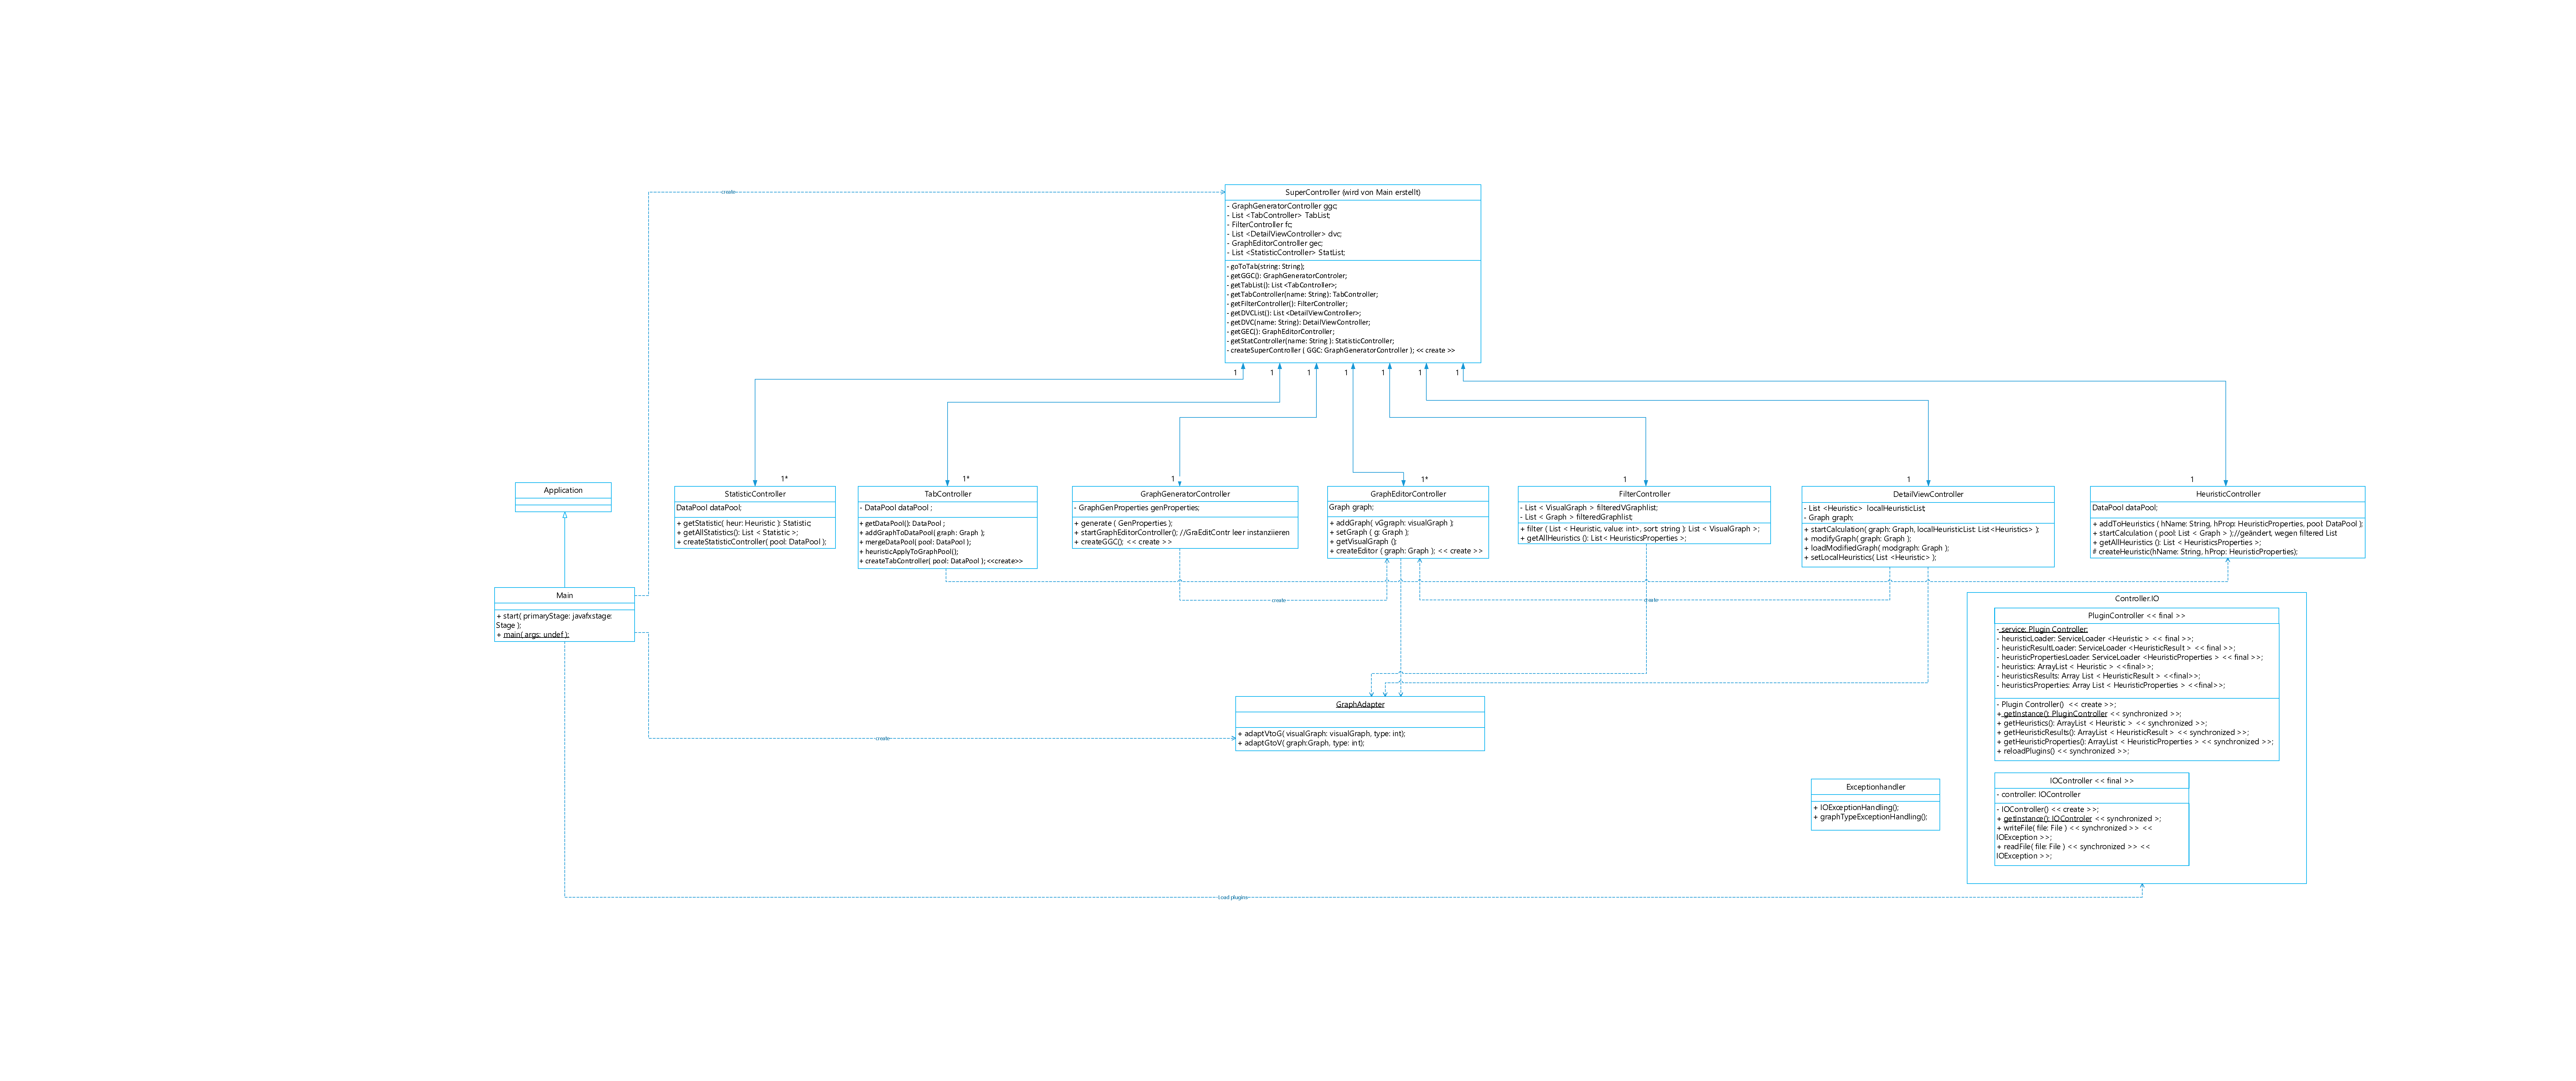
\includegraphics[width=\textwidth]{abbildungen/ControllerOhneMethodenBeschreibung.pdf}
\caption{Controller }
	\label{img:controller}
	\end{figure}

\myclass{SuperController}

\textbf{Description}

The SuperController has one or more instances of theGrapgGeneratorController, List of TabController, GraphEditorController. \newline
\textbf{Documentation}
\begin{enumerate}[+]
	\item{
	\textbf{SuperController} \newline
	Constructor: Creates a SuperController and gives him immedeately a GraphGeneratorController instance.  \newline
	\textbf{@param GGC} The Param GGC is the instance of a GraphGeneratorController. \newline
	}

	\item{
	\textbf{getGGC} \newline
	\textbf{@return} GraphGeneratorController. \newline

	}
	\item{
	\textbf{createGEC} \newline
	Creates a new GraphEditorController with(out) a graph to display.  \newline
	\textbf{@param pool} The DataPool, where the created graph from the user will be added. \newline
	\textbf{@param graphl} The Graphl, that should be modified. \newline
	}
	\item{
	\textbf{getTabList} \newline
	\textbf{@return} List <TabController>. \newline
	}
	\item{
	\textbf{getTabController} \newline
	\textbf{@param name} name is the PreviewTab identifier, with it, the SuperController can \newline
	identify the current TabController, the User is working on. \newline
	\textbf{@return} TabController. \newline
	}
	\item{
	\textbf{getGEC} \newline
	\textbf{@return} GraphEditorController. \newline
	}
	\item{
	\textbf{createTabController} \newline
	Creates a new preview tab, with a graph liast and a heuristics list.  \newline
	\textbf{@param graphList} List of graphs that should be taken to the new tab. \newline
	\textbf{@param heurList} List of heuristics that should be taken to the new tab. \newline
	\textbf{@return} TabController. \newline
	}
	\item{
	\textbf{createTabController} \newline
	Creates a new preview tab with its own DataPool, and calls the GrapgGeneratorController to generate graphs for the DataPool and it will show the graphs in the preview Tab.  \newline
	\textbf{@param GgenPropertiest} The properties, that dictates how the random graph generation generates graphsö. \newline
	\textbf{@return} TabController. \newline
	}
	\item[-]{
		\textbf{PRIVATEMETHODE} etc
	}
\end{enumerate}

\myclass{StatisticController}

\textbf{Description}

Reads the statistics for a heuristic out of the Model and collects them to show it to the View.

\textbf{Documentation}
\begin{enumerate}[+]
	\item{
	\textbf{StatisticController} \newline
	Constructor: Creates a StatisticController and gets himself a DataPool.
	\textbf{@param pool} The DataPool, that the StatisticController belongs to. \newline
}
	\item{
	\textbf{getAllStatistics} \newline
	\textbf{@return} List <Statistic >. \newline
}
	\item{
	\textbf{getStatistic} \newline
	\textbf{@param heur} heur is the Name of the Heuristic, that you want the statistics from. \newline
	\textbf{@return} Statistic. \newline
}
	\item[-]{
		\textbf{PRIVATEMETHODE} etc
	}
\end{enumerate}

\myclass{TabController}

\textbf{Beschreibung}

The Controller of exactly one Preview Tab in the View, that manages the DataPool of this Preview Tab.

\textbf{Dokumentation}
\begin{enumerate}[+]
	\item{
	\textbf{TabController} \newline
	Constructor: Creates a new TabController and connects it with an own DataPool, it also creates an own StatisticController. \newline
	\textbf{@param tabnamel} The name of this TabController. \newline
	\textbf{@param pool} The DataPool, that belongs to the TabController. \newline
}
	\item{
	\textbf{getDVCList} \newline
	\textbf{@return} List <DetailViewController>. \newline
}
	\item{
	\textbf{getDVC} \newline
	\textbf{@param name} The name is the DetailViewController identifier, with it, theTabController can \newline
	identify the current DetailViewController, the User is working on. \newline
	\textbf{@return} DetailViewController. \newline
	}
	\item{
	\textbf{getDataPool} \newline
	\textbf{@return} DataPool \newline
}
	\item{
	\textbf{addGraphToDataPool} \newline
	Adds one Graph to the DataPool, that belongs to the TabController instance. \newline
	\textbf{@param graph} The graph that should be added to the DataPool. \newline
	\textbf{@throws EXCEPTION} if the type of the Graph is not of the same graph type in the DataPool. \newline
}
	\item{
	\textbf{mergeDataPool} \newline
	Merges two DataPools under one of the two TabController. The other TabController with its DataPool remains untouched. \newline
	\textbf{@param pool} The DataPool, that should be copied. \newline
	\textbf{@throws EXCEPTION} if the graph type of both DataPools is not equal.
}
	\item{
	\textbf{getStatisticController} \newline
	\textbf{@return} StatisticController \newline
}
	\item{
	\textbf{getHeuristicController} \newline
	\textbf{@return} HeuristicController \newline
}
	\item{
	\textbf{getFilterController} \newline
	\textbf{@return} FilterController \newline
}
	\item{
	\textbf{heuristicApplyToDataPool} \newline
	Calls the HeuristicController to collor the graphs. \newline
}
	\item{
	\textbf{createHeuristicController} \newline
	Instanciates a HeuristicController and gives him a DataPool.
	\textbf{@param pool} The given DataPool. \newline
}
	\item{
	\textbf{createDetailViewController} \newline
	Instanciates a DetailViewController and gives him a graph to display with all heuristics, that tried to collor it.
	\textbf{@param graphPositionl} The position of the graph in the graph list in the given DataPool. \newline
}
	\item{
	\textbf{createFilterController} \newline
	Instanciates a FilterController and gives him a DataPool.
	\textbf{@param pool} The given DataPool. \newline
}

	\item[-]{
		\textbf{PRIVATEMETHODE} etc
	}
\end{enumerate}
\myclass{GraphGeneratorController}

\textbf{Beschreibung}

The controller for the graph generation communication between the view and the GraphBuilder in the Model.

\textbf{Dokumentation}
\begin{enumerate}[+]
	\item{
	\textbf{GraphGeneratorController} \newline
	Constructor: Creates a GraphGeneratorController. \newline
}
	\item{
	\textbf{generate} \newline
	Commands the GraphBuilder to create random graphs with specific properties. \newline
	\textbf{@param genProperties} The properties, that restrict the randomnes of the GraphBuilder.\newline

}

	\item{
	\textbf{createManuallyGraph} \newline
	Creates an empty GraphEditorController, that adds that manually generated graph from a user.\newline
	It calls the SuperController to start the method createGEC without a DataPool and without a graph.\newline

}
	\item[-]{
		\textbf{PRIVATEMETHODE} etc
	}
\end{enumerate}
\myclass{GraphEditorController}

\textbf{Beschreibung}

Manages the manipulated or created graph by the user and adds it to the right DataPool. \newline

\textbf{Dokumentation}
\begin{enumerate}[+]
	\item{
	\textbf{GraphEditorController} \newline
	Constructor: Creates a GraphEditorController and it will get a DataPool instance. When it was created by the GraphGeneratorController, it will create an GraphEditorController without a graph. \newline
	If it was created by the DetailViesController, it will get a graph to the new instance. \newline
}
	\item{
	\textbf{setGraph} \newline
	Sets the graph of this instance. \newline
	\textbf{@param g} The graph, that belongs to this instance.\newline
}

	\item{
	\textbf{addGraph} \newline
	Adapts the created visualGraph to a Graph and adds the created graph to the DataPool. If there is no DataPool, it will create a new one. \newline
	\textbf{@param vGraph} The created visualGraph. \newline
}
	\item{
	\textbf{getVisualGraph} \newline
	Returns the Graph of this instance as a visualGraph. \newline
}
	\item[-]{
		\textbf{PRIVATEMETHODE} etc
	}
\end{enumerate}
\myclass{FilterController}

\textbf{Beschreibung}

Controlls the filter set by the user and manages the filtered graph pool and the graph pool in the DataPool. \newline

\textbf{Dokumentation}
\begin{enumerate}[+]
	\item{
	\textbf{createFilterController} \newline
	Constructor: Creates a FilterrController and it will get a DataPool instance. \newline
}
	\item{
	\textbf{filter} \newline
	Filters the graph list from the DataPool. \newline
	\textbf{@param List <Heuristic, value: int>} It determines how the list will be filtered. \newline
	\textbf{@param sort} It determines how list will be sorted (decending, ascending ...). \newline
	\textbf{@return} returns List <VisualGraph>, the DataPool remains untouched. \newline
	\textbf{@throws EXCEPTION} if filter and sort are contradictory.\newline
}
	\item{
	\textbf{getAllHeuristics} \newline
	Returns all properties of the used heuristics and the heuristic name is also a heuristic property. \newline
	\textbf{@return} returns List <HeuristicProperties> \newline
}
	\item[-]{
		\textbf{PRIVATEMETHODE} etc
	}
\end{enumerate}
\myclass{DetailViewController}

\textbf{Beschreibung}

Manages the chosen graph and the heuristics that only apply to this graph, the so called local heuristics. \newline

\textbf{Dokumentation}
\begin{enumerate}[+]
	\item{
	\textbf{startCalculation} \newline
	Applies the local Heuristics to the one graph in the DetailView. \newline
	\textbf{@param graph} The graph that get colloerd by the local heuristics. \newline
	\textbf{@param localHeuristicList} The list of local heuristics, that collors the one graph.
}

	\item{
	\textbf{modifyGraph} \newline
	Creates a GraphEditorController instance with the one graph. \newline
	\textbf{@param graph} The graph that should be modified. \newline
}
	\item{
	\textbf{loadModifiedGraph} \newline
	Loads the modified graph into the DataPool and in to the DetailViewController. \newline
	\textbf{@param modgraph} The modified graph. \newline
}
	\item{
	\textbf{addLocalHeuristics} \newline
	Adds the local heuristics chosen by the user to the localHeuristics. \newline
	\textbf{@param List <Heuristic>} The local Heuristics. \newline
}
	\item{
	\textbf{DetailViewController} \newline
	Creates a new Detail View Controller and creates an empty localHeuristicsList. \newline
	\textbf{@param graph} The graph, thatshouldbe loaded in to the DetailViewController. \newline
}
	\item[-]{
		\textbf{PRIVATEMETHODE} etc
	}
\end{enumerate}
\myclass{HeuristicController}

\textbf{Beschreibung}

Manages the chosen graph and the heuristics that only apply to this graph, the so called local heuristics. \newline

\textbf{Dokumentation}
\begin{enumerate}[+]
	\item{
	\textbf{HeuristicController} \newline
	Creates a HeuristicController and gives him a DataPool. \newline
	\textbf{@param pool} The DataPool to give. \newline
}
	\item{
	\textbf{addToHeuristics} \newline
	Applies the chosen heuristics to the heuristic pool in the DataPool. Calls the createHeuristics method. \newline
	\textbf{@param hName } The name of the heuristic. \newline
	\textbf{@param hProp } The properties of the heuristic. \newline
	\textbf{@param pool } The DataPool, where the heuristics belong. \newline
}
	\item{
	\textbf{startCalculation} \newline
	Commands the Heuristics to calculate their results on the graph pool. \newline
	\textbf{@param pool} The graph list.  \newline
	\textbf{@param hpool} The heuristicList of the DataPool, that should calculate the result on the graph list.  \newline
}
	\item{
	\textbf{getAllHeuristics} \newline
	Returns all possible Heuristics. \newline
	\textbf{@return} returns List <HeuristicsProperties>.  \newline
}
	\item[\#]{
	\item{
	\textbf{createHeuristics} \newline
	Get invoked by addToHeuristics and commands the model to create a new heuristic. \newline
	\textbf{@param hName} The heuristic name. \newline
	\textbf{@param hProp} The heuristic properties. \newline
}}
\end{enumerate}
	%Siehe Berard.
	
	\subsection{View-Controller}
	%\begin{enumerate}
	\subsubsection{Allgemein}
		%Einleitung
		Der Graphic-Controller oder unter JavaFx üblicherweise auch FxController ist der Teil eines JavaFx-Programms der direkt mit dem von der FXML-Datei bereitgestellten GUI verknüpft ist.
		Der FxController ist somit ein Separater Teil des Controllers, der sich lediglich mit der GUI beschäftigt und die getätigten Eingaben an die richtigen Stellen im allgemeinen Controller weitergibt.
			Dies bringt den Vorteil, dass der allgemeine Controller keine Kenntnisse über die GUI benötigt und losgelöst von dieser funktionieren kann.
			Dadurch ist auch die Modularität in diesem Teil des Entwurfs gewährleistet.
	
	\subsubsection{Entwurf}
		%Hier das ClassDiagram_ViewController UML einfügen.
		\begin{figure}
	\centering	
%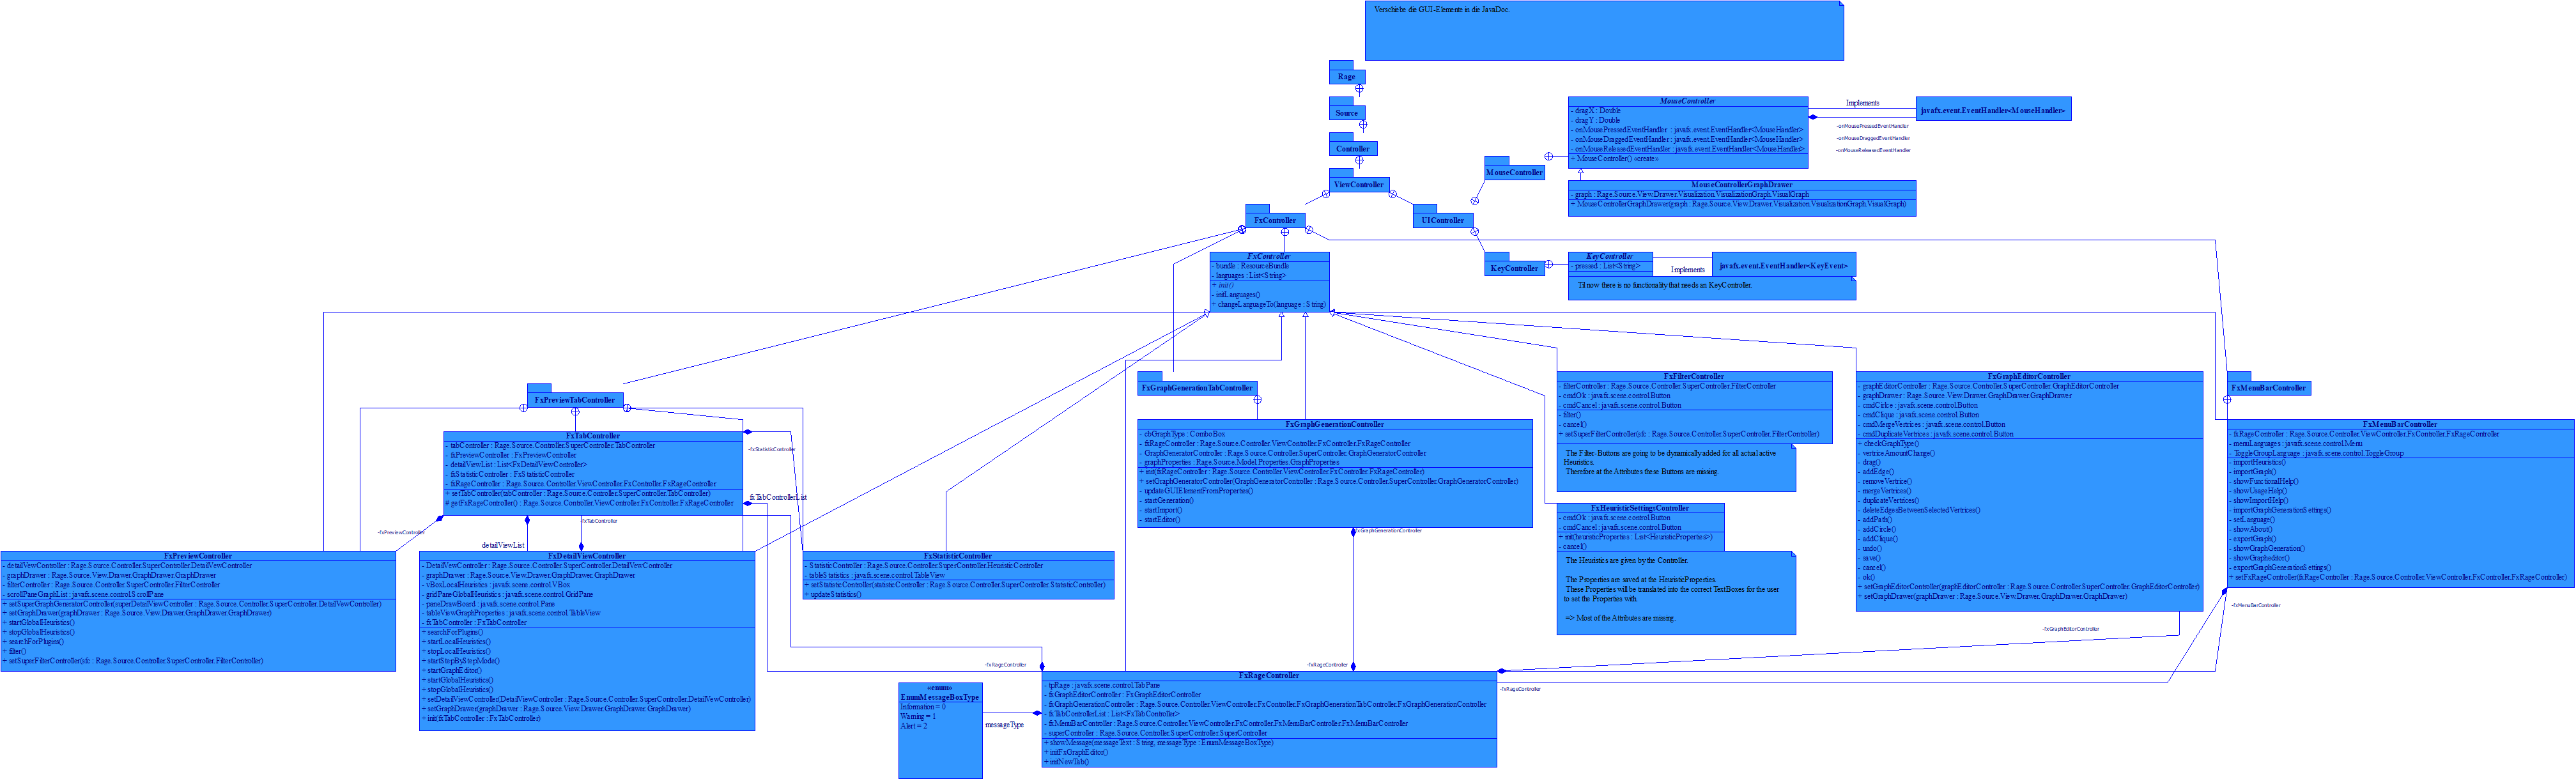
\includegraphics[angle=270,width=0.5\textwidth]{ClassDiagram_ViewController.png}
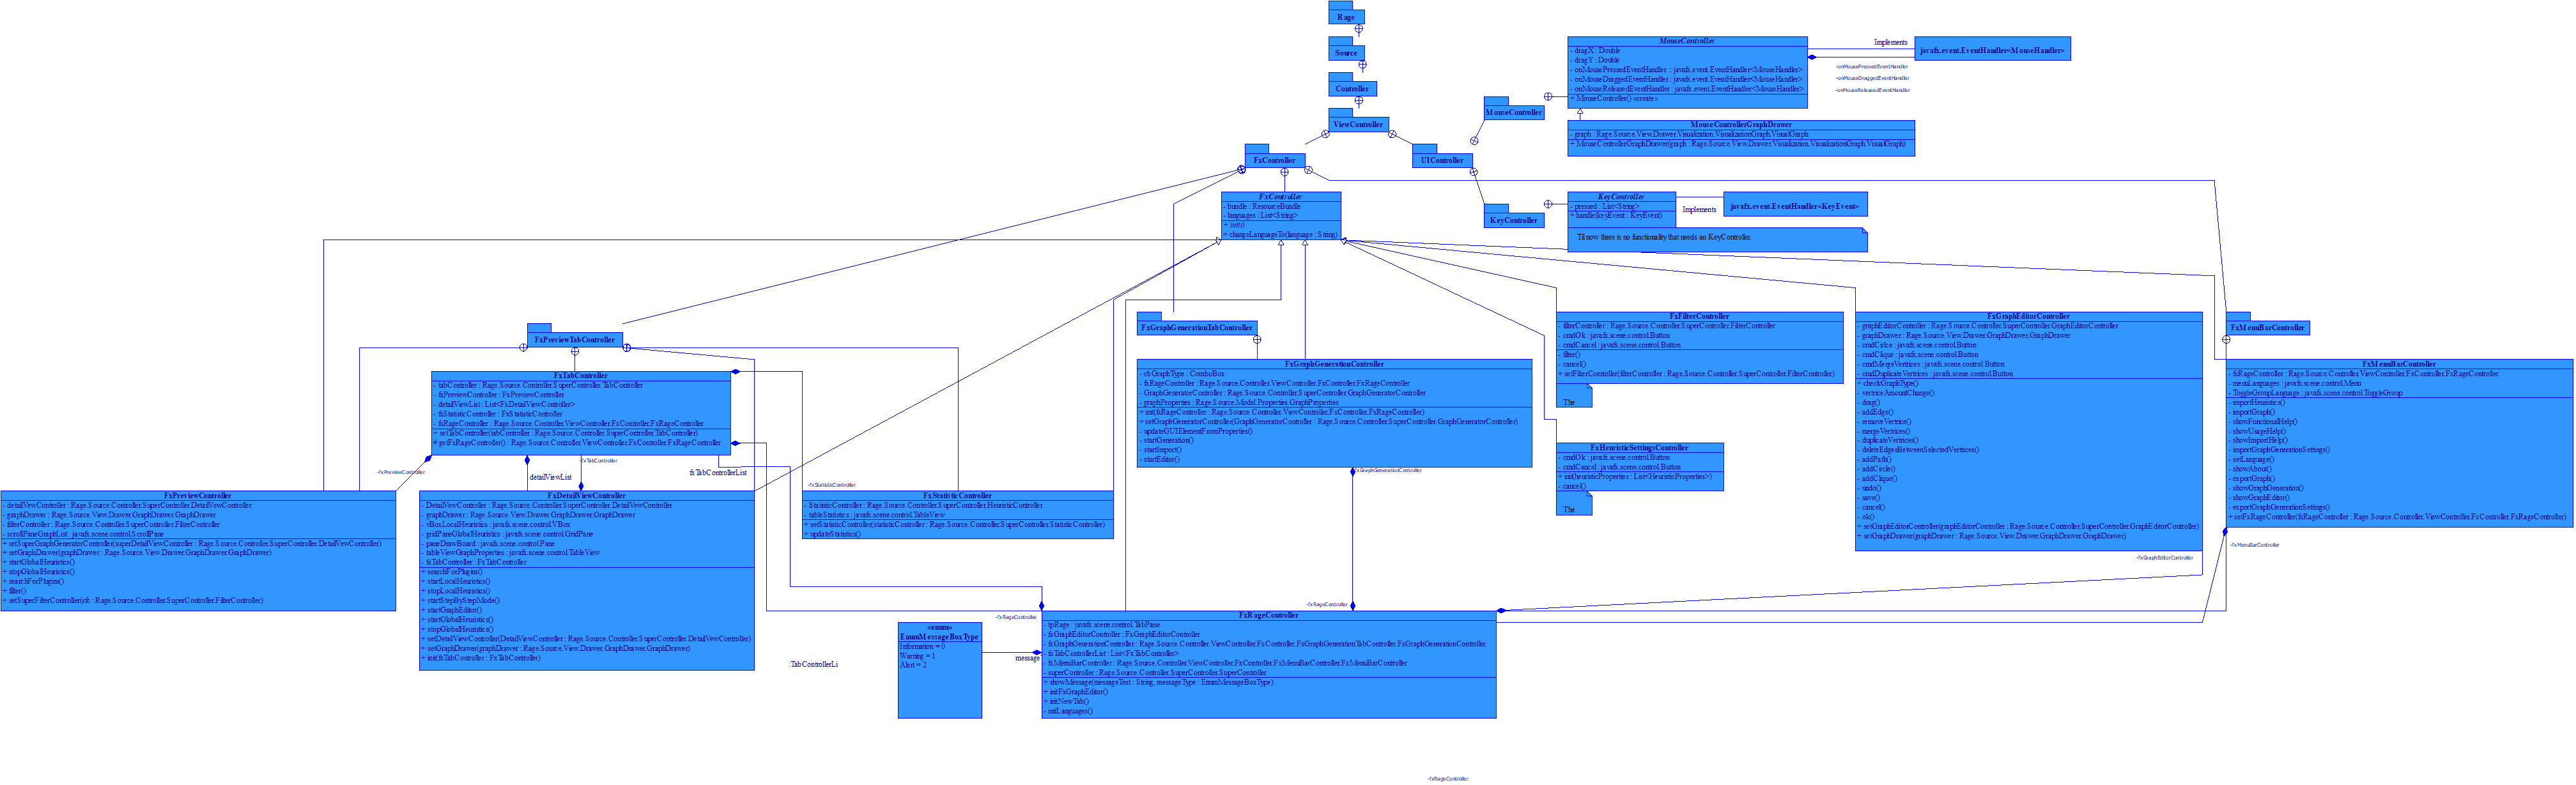
\includegraphics[width=\textwidth]{abbildungen/ClassDiagram_ViewController.png}
\caption{ViewController}
\label{img:viewcontroller}
	\end{figure}
		
		%TODO View-Controller
	
	%\end{enumerate}
	

	%Entwurf
	
	\section{Resources}
	%\begin{enumerate}
	\subsection{Allgemein}
		%Einleitung
		Die Ressourcen sind alle Dateien, die nicht in direktem Zusammenhang mit der Funktionalität und des Programms stehen und keinen Einfluss auf den Ablauf haben.
		Hierunter fallen meist Bilder, wie Icons, oder auch andere Mediendateien und vieles mehr.
		Diese Dateien muss unser Programm aus externen Stellen ziehen.
	
	\subsection{Entwurf} 
		%Entwurf
		Diese Daten werden getrennt vom Programmcode abgelegt und dann bei Bedarf aus der vordefinierten Stelle vom Programm eingeladen.
		
		%Aufbau
		%UML Diagramm der Ressourcen zum Überblick hier einfügbar. :)
		
		\mypackage{Resources}
		This contains all the Resources that are needed for the Project.
		
		\begin{enumerate}[*]
			\item{
				\textbf{FXML} \newline
				This contains all the FXML files for the GUI.
				They are arranged in different Sub-Folders to separate.
				\newline
			}
			\subitem{
				\textbf{Main} \newline
			}
			\subsubitem{
				\textbf{StartTab} \newline
			}
			\subsubitem{
				\textbf{Preview} \newline
			}
			\subsubitem{
				\textbf{GraphGeneration} \newline
			}
			
			\subitem{
				\textbf{MenuBar} \newline
			}
			\subitem{
				\textbf{Editor} \newline
			}
			\subitem{
				\textbf{Popups} \newline
			}
			
			\item{
				\textbf{Pictrues} \newline
				This contains all the Pictures used at the GUI organized by sub-Folders.
			}
			\subsubitem{
				\textbf{Icons} \newline
				This contains all Icons for the Buttons, ... of the GUI.
			}
			\subsubitem{
				\textbf{Logo} \newline
				This contains all Logos used at the GUI.
			}
			\item{
				\textbf{Sound} \newline
				This contains all the Sounds that can be played by default.
			}
			\item{
				\textbf{StyleSheets} \newline
				This Contains all the CSS-Files for the GUI.
			}
			\item{
				\textbf{Plugins} \newline
				This Contains all the Plugins the User could add to the Rage-Program.
				By Default, there are the Plugins for the TC and EFL that we should implement.
			}
			\item{
				\textbf{Log} \newline
				Contains the Log-Files.
			}
		\end{enumerate}
	%}
	%\end{enumerate}
	
%\input{controller2}
	\section{Input-Output}
	\mypackage{IO}

This package contains classes for input, output and plugin loading.

\myclass{PluginController}

\textbf{Beschreibung}

Loads all Heuristic, HeuristicResult and HeuristicProperties classes using the ServiceLoader class. It uses the singelton design pattern.

\textbf{Dokumentation}
\begin{enumerate}[+]
	\item{
		\textbf{getInstance():PluginController} \newline
		This method is the only way to access the PluginController. Creates a new PluginController if it does not exist. \newline
		\textbf{@return} returns the PluginController itself. \newline
	}
	\item{
		\textbf{getHeuristics():ArrayList<Heuristic> } \newline
		Loads all Heuristic classes if they are not already loaded. \newline
		\textbf{@return} returns a list with all Heuristics. \newline
	}
	\item{
		\textbf{getHeuristicResults():ArrayList<HeuristicResult>} \newline
		Loads all HeuristicResult classes if they are not already loaded. \newline
		\textbf{@return} returns a list with all HeuristicResult classes. \newline
	}
	\item{
		\textbf{getHeuristicProperties():ArrayList<HeuristicProperties>} \newline
		Loads all HeuristicProperties classes if they are not already loaded. \newline
		\textbf{@return} returns a list with all HeuristicProperties classes. \newline
	}
	\item{
		\textbf{reloadPlugins()} \newline
		Clears the pluginlists and then loads all plugins. \newline
	}
\end{enumerate}

\myclass{IOController}

\textbf{Beschreibung}

Saves and loads the data of a single view tab. The file has the extension \glqq.RAGE\grqq. It uses the singelton design pattern.

\textbf{Dokumentation}
\begin{enumerate}[+]
	\item{
		\textbf{getInstance():IOController} \newline
		This method is the only way to access the IOController. Creates a new IOController if it does not exist. \newline
		\textbf{@return} returns the IOController itself. \newline
	}
	\item{
		\textbf{writeFile(File file)} \newline
		Writes a RAGE file to the disk. \newline
		\textbf{@param file} Information about the file. \newline
		\textbf{@throws IOException} if saving fails print: \glqq Error while saving the file.\grqq.
	}
	\item{
		\textbf{readFile(File file)} \newline
		Reads a RAGE file from the disk and sends the content to the model. \newline
		\textbf{@param file} Information about the file. \newline
		\textbf{@throws IOException} if loading fails print: \glqq Error while loading the file.\grqq.
	}
\end{enumerate}
	\section{Utils}
	\section{Addendum: Heuristiken}
	\section{Addendum: RAGE-Datenformate}
	
\end{document}
